\documentclass[10pt, oneside]{article} 
\usepackage{amsmath, amsthm, amssymb, calrsfs, wasysym, verbatim, bbm, color, graphics, geometry, esint, float}


\geometry{tmargin=.75in, bmargin=.75in, lmargin=.75in, rmargin = .75in}  

\newcommand{\bbR}{\mathbb{R}}
\newcommand{\bbC}{\mathbb{C}}
\newcommand{\bbZ}{\mathbb{Z}}
\newcommand{\bbP}{\mathbb{P}}
\newcommand{\bbN}{\mathbb{N}}
\newcommand{\bbQ}{\mathbb{Q}}
\newcommand{\Cdot}{\boldsymbol{\cdot}}
\newcommand{\scA}{\mathscr{A}}
\newcommand{\curl}{\text{curl}}
\newcommand{\Ind}{\text{Ind}}
\newcommand{\Log}{\text{Log}}
\newcommand{\hcap}{\text{hcap}}
\newcommand{\rad}{\text{rad}}


\newcommand{\sm}{\setminus}

\theoremstyle{definition}
\newtheorem{exmp}{Example}[section]
\newtheorem{thm}{Theorem}
\newtheorem{defn}{Definition}
\newtheorem{prop}{Proposition}
\newtheorem{conv}{Convention}
\newtheorem{rem}{Remark}
\newtheorem{lem}{Lemma}
\newtheorem{cor}{Corollary}
% Copyright 2021 Paolo Adajar (padajar.com, paoloadajar@mit.edu)
% 
% Permission is hereby granted, free of charge, to any person obtaining a copy of this software and associated documentation files (the "Software"), to deal in the Software without restriction, including without limitation the rights to use, copy, modify, merge, publish, distribute, sublicense, and/or sell copies of the Software, and to permit persons to whom the Software is furnished to do so, subject to the following conditions:
%
% The above copyright notice and this permission notice shall be included in all copies or substantial portions of the Software.
% 
% THE SOFTWARE IS PROVIDED "AS IS", WITHOUT WARRANTY OF ANY KIND, EXPRESS OR IMPLIED, INCLUDING BUT NOT LIMITED TO THE WARRANTIES OF MERCHANTABILITY, FITNESS FOR A PARTICULAR PURPOSE AND NONINFRINGEMENT. IN NO EVENT SHALL THE AUTHORS OR COPYRIGHT HOLDERS BE LIABLE FOR ANY CLAIM, DAMAGES OR OTHER LIABILITY, WHETHER IN AN ACTION OF CONTRACT, TORT OR OTHERWISE, ARISING FROM, OUT OF OR IN CONNECTION WITH THE SOFTWARE OR THE USE OR OTHER DEALINGS IN THE SOFTWARE.

\usepackage{fullpage}
\usepackage{enumitem}
\usepackage{amsfonts, amssymb, amsmath,amsthm}
\usepackage{mathtools}
\usepackage[pdftex, pdfauthor={\name}, pdftitle={\classnum~\assignment}]{hyperref}
\usepackage[dvipsnames]{xcolor}
\usepackage{bbm}
\usepackage{graphicx}
\usepackage{mathrsfs}
\usepackage{pdfpages}
\usepackage{tabularx}
\usepackage{pdflscape}
\usepackage{makecell}
\usepackage{booktabs}
\usepackage{natbib}
\usepackage{caption}
\usepackage{subcaption}
\usepackage{physics}
\usepackage[many]{tcolorbox}
\usepackage{version}
\usepackage{ifthen}
\usepackage{cancel}
\usepackage{listings}
\usepackage{courier}

\usepackage{tikz}
\usepackage{istgame}

\hypersetup{
	colorlinks=true,
	linkcolor=blue,
	filecolor=magenta,
	urlcolor=blue,
}

\setlength{\parindent}{0mm}
\setlength{\parskip}{2mm}

\setlist[enumerate]{label=({\alph*})}
\setlist[enumerate, 2]{label=({\roman*})}

\allowdisplaybreaks[1]

\newcommand{\psetheader}{
	\ifthenelse{\isundefined{\collaborators}}{
		\begin{center}
			{\setlength{\parindent}{0cm} \setlength{\parskip}{0mm}
				
				{\textbf{\classnum~\semester:~\assignment} \hfill \name}
				
				\subject \hfill \href{mailto:\email}{\tt \email}
				
				Instructor(s):~\instructors \hfill Due Date:~\duedate	
				
				\hrulefill}
		\end{center}
	}{
		\begin{center}
			{\setlength{\parindent}{0cm} \setlength{\parskip}{0mm}
				
				{\textbf{\classnum~\semester:~\assignment} \hfill \name\footnote{Collaborator(s): \collaborators}}
				
				\subject \hfill \href{mailto:\email}{\tt \email}
				
				Instructor(s):~\instructors \hfill Due Date:~\duedate	
				
				\hrulefill}
		\end{center}
	}
}

\renewcommand{\thepage}{\classnum~\assignment \hfill \arabic{page}}

\makeatletter
\def\points{\@ifnextchar[{\@with}{\@without}}
\def\@with[#1]#2{{\ifthenelse{\equal{#2}{1}}{{[1 point, #1]}}{{[#2 points, #1]}}}}
\def\@without#1{\ifthenelse{\equal{#1}{1}}{{[1 point]}}{{[#1 points]}}}
\makeatother

\newtheoremstyle{theorem-custom}%
{}{}%
{}{}%
{\itshape}{.}%
{ }%
{\thmname{#1}\thmnumber{ #2}\thmnote{ (#3)}}

\theoremstyle{theorem-custom}

\newtheorem{theorem}{Theorem}
\newtheorem{lemma}[theorem]{Lemma}
\newtheorem{example}[theorem]{Example}

\newenvironment{problem}[1]{\color{black} #1}{}

\newenvironment{solution}{%
	\leavevmode\begin{tcolorbox}[breakable, colback=green!5!white,colframe=green!75!black, enhanced jigsaw] \proof[\scshape Solution:] \setlength{\parskip}{2mm}%
	}{\renewcommand{\qedsymbol}{$\blacksquare$} \endproof \end{tcolorbox}}

\newenvironment{reflection}{\begin{tcolorbox}[breakable, colback=black!8!white,colframe=black!60!white, enhanced jigsaw, parbox = false]\textsc{Reflections:}}{\end{tcolorbox}}

\newcommand{\qedh}{\renewcommand{\qedsymbol}{$\blacksquare$}\qedhere}

\definecolor{mygreen}{rgb}{0,0.6,0}
\definecolor{mygray}{rgb}{0.5,0.5,0.5}
\definecolor{mymauve}{rgb}{0.58,0,0.82}

% from https://github.com/satejsoman/stata-lstlisting
% language definition
\lstdefinelanguage{Stata}{
	% System commands
	morekeywords=[1]{regress, reg, summarize, sum, display, di, generate, gen, bysort, use, import, delimited, predict, quietly, probit, margins, test},
	% Reserved words
	morekeywords=[2]{aggregate, array, boolean, break, byte, case, catch, class, colvector, complex, const, continue, default, delegate, delete, do, double, else, eltypedef, end, enum, explicit, export, external, float, for, friend, function, global, goto, if, inline, int, local, long, mata, matrix, namespace, new, numeric, NULL, operator, orgtypedef, pointer, polymorphic, pragma, private, protected, public, quad, real, return, rowvector, scalar, short, signed, static, strL, string, struct, super, switch, template, this, throw, transmorphic, try, typedef, typename, union, unsigned, using, vector, version, virtual, void, volatile, while,},
	% Keywords
	morekeywords=[3]{forvalues, foreach, set},
	% Date and time functions
	morekeywords=[4]{bofd, Cdhms, Chms, Clock, clock, Cmdyhms, Cofc, cofC, Cofd, cofd, daily, date, day, dhms, dofb, dofC, dofc, dofh, dofm, dofq, dofw, dofy, dow, doy, halfyear, halfyearly, hh, hhC, hms, hofd, hours, mdy, mdyhms, minutes, mm, mmC, mofd, month, monthly, msofhours, msofminutes, msofseconds, qofd, quarter, quarterly, seconds, ss, ssC, tC, tc, td, th, tm, tq, tw, week, weekly, wofd, year, yearly, yh, ym, yofd, yq, yw,},
	% Mathematical functions
	morekeywords=[5]{abs, ceil, cloglog, comb, digamma, exp, expm1, floor, int, invcloglog, invlogit, ln, ln1m, ln, ln1p, ln, lnfactorial, lngamma, log, log10, log1m, log1p, logit, max, min, mod, reldif, round, sign, sqrt, sum, trigamma, trunc,},
	% Matrix functions
	morekeywords=[6]{cholesky, coleqnumb, colnfreeparms, colnumb, colsof, corr, det, diag, diag0cnt, el, get, hadamard, I, inv, invsym, issymmetric, J, matmissing, matuniform, mreldif, nullmat, roweqnumb, rownfreeparms, rownumb, rowsof, sweep, trace, vec, vecdiag, },
	% Programming functions
	morekeywords=[7]{autocode, byteorder, c, _caller, chop, abs, clip, cond, e, fileexists, fileread, filereaderror, filewrite, float, fmtwidth, has_eprop, inlist, inrange, irecode, matrix, maxbyte, maxdouble, maxfloat, maxint, maxlong, mi, minbyte, mindouble, minfloat, minint, minlong, missing, r, recode, replay, return, s, scalar, smallestdouble,},
	% Random-number functions
	morekeywords=[8]{rbeta, rbinomial, rcauchy, rchi2, rexponential, rgamma, rhypergeometric, rigaussian, rlaplace, rlogistic, rnbinomial, rnormal, rpoisson, rt, runiform, runiformint, rweibull, rweibullph,},
	% Selecting time-span functions
	morekeywords=[9]{tin, twithin,},
	% Statistical functions
	morekeywords=[10]{betaden, binomial, binomialp, binomialtail, binormal, cauchy, cauchyden, cauchytail, chi2, chi2den, chi2tail, dgammapda, dgammapdada, dgammapdadx, dgammapdx, dgammapdxdx, dunnettprob, exponential, exponentialden, exponentialtail, F, Fden, Ftail, gammaden, gammap, gammaptail, hypergeometric, hypergeometricp, ibeta, ibetatail, igaussian, igaussianden, igaussiantail, invbinomial, invbinomialtail, invcauchy, invcauchytail, invchi2, invchi2tail, invdunnettprob, invexponential, invexponentialtail, invF, invFtail, invgammap, invgammaptail, invibeta, invibetatail, invigaussian, invigaussiantail, invlaplace, invlaplacetail, invlogistic, invlogistictail, invnbinomial, invnbinomialtail, invnchi2, invnF, invnFtail, invnibeta, invnormal, invnt, invnttail, invpoisson, invpoissontail, invt, invttail, invtukeyprob, invweibull, invweibullph, invweibullphtail, invweibulltail, laplace, laplaceden, laplacetail, lncauchyden, lnigammaden, lnigaussianden, lniwishartden, lnlaplaceden, lnmvnormalden, lnnormal, lnnormalden, lnwishartden, logistic, logisticden, logistictail, nbetaden, nbinomial, nbinomialp, nbinomialtail, nchi2, nchi2den, nchi2tail, nF, nFden, nFtail, nibeta, normal, normalden, npnchi2, npnF, npnt, nt, ntden, nttail, poisson, poissonp, poissontail, t, tden, ttail, tukeyprob, weibull, weibullden, weibullph, weibullphden, weibullphtail, weibulltail,},
	% String functions 
	morekeywords=[11]{abbrev, char, collatorlocale, collatorversion, indexnot, plural, plural, real, regexm, regexr, regexs, soundex, soundex_nara, strcat, strdup, string, strofreal, string, strofreal, stritrim, strlen, strlower, strltrim, strmatch, strofreal, strofreal, strpos, strproper, strreverse, strrpos, strrtrim, strtoname, strtrim, strupper, subinstr, subinword, substr, tobytes, uchar, udstrlen, udsubstr, uisdigit, uisletter, ustrcompare, ustrcompareex, ustrfix, ustrfrom, ustrinvalidcnt, ustrleft, ustrlen, ustrlower, ustrltrim, ustrnormalize, ustrpos, ustrregexm, ustrregexra, ustrregexrf, ustrregexs, ustrreverse, ustrright, ustrrpos, ustrrtrim, ustrsortkey, ustrsortkeyex, ustrtitle, ustrto, ustrtohex, ustrtoname, ustrtrim, ustrunescape, ustrupper, ustrword, ustrwordcount, usubinstr, usubstr, word, wordbreaklocale, worcount,},
	% Trig functions
	morekeywords=[12]{acos, acosh, asin, asinh, atan, atanh, cos, cosh, sin, sinh, tan, tanh,},
	morecomment=[l]{//},
	% morecomment=[l]{*},  // `*` maybe used as multiply operator. So use `//` as line comment.
	morecomment=[s]{/*}{*/},
	% The following is used by macros, like `lags'.
	morestring=[b]{`}{'},
	% morestring=[d]{'},
	morestring=[b]",
	morestring=[d]",
	% morestring=[d]{\\`},
	% morestring=[b]{'},
	sensitive=true,
}

\lstset{ 
	backgroundcolor=\color{white},   % choose the background color; you must add \usepackage{color} or \usepackage{xcolor}; should come as last argument
	basicstyle=\footnotesize\ttfamily,        % the size of the fonts that are used for the code
	breakatwhitespace=false,         % sets if automatic breaks should only happen at whitespace
	breaklines=true,                 % sets automatic line breaking
	captionpos=b,                    % sets the caption-position to bottom
	commentstyle=\color{mygreen},    % comment style
	deletekeywords={...},            % if you want to delete keywords from the given language
	escapeinside={\%*}{*)},          % if you want to add LaTeX within your code
	extendedchars=true,              % lets you use non-ASCII characters; for 8-bits encodings only, does not work with UTF-8
	firstnumber=0,                % start line enumeration with line 1000
	frame=single,	                   % adds a frame around the code
	keepspaces=true,                 % keeps spaces in text, useful for keeping indentation of code (possibly needs columns=flexible)
	keywordstyle=\color{blue},       % keyword style
	language=Octave,                 % the language of the code
	morekeywords={*,...},            % if you want to add more keywords to the set
	numbers=left,                    % where to put the line-numbers; possible values are (none, left, right)
	numbersep=5pt,                   % how far the line-numbers are from the code
	numberstyle=\tiny\color{mygray}, % the style that is used for the line-numbers
	rulecolor=\color{black},         % if not set, the frame-color may be changed on line-breaks within not-black text (e.g. comments (green here))
	showspaces=false,                % show spaces everywhere adding particular underscores; it overrides 'showstringspaces'
	showstringspaces=false,          % underline spaces within strings only
	showtabs=false,                  % show tabs within strings adding particular underscores
	stepnumber=2,                    % the step between two line-numbers. If it's 1, each line will be numbered
	stringstyle=\color{mymauve},     % string literal style
	tabsize=2,	                   % sets default tabsize to 2 spaces
%	title=\lstname,                   % show the filename of files included with \lstinputlisting; also try caption instead of title
	xleftmargin=0.25cm
}
\newcommand{\bA}{\mathbf{A}}
\newcommand{\bB}{\mathbf{B}}
\newcommand{\bC}{\mathbf{C}}
\newcommand{\bD}{\mathbf{D}}
\newcommand{\bE}{\mathbf{E}}
\newcommand{\bF}{\mathbf{F}}
\newcommand{\bG}{\mathbf{G}}
\newcommand{\bH}{\mathbf{H}}
\newcommand{\bI}{\mathbf{I}}
\newcommand{\bJ}{\mathbf{J}}
\newcommand{\bK}{\mathbf{K}}
\newcommand{\bL}{\mathbf{L}}
\newcommand{\bM}{\mathbf{M}}
\newcommand{\bN}{\mathbf{N}}
\newcommand{\bO}{\mathbf{O}}
\newcommand{\bP}{\mathbf{P}}
\newcommand{\bQ}{\mathbf{Q}}
\newcommand{\bR}{\mathbf{R}}
\newcommand{\bS}{\mathbf{S}}
\newcommand{\bT}{\mathbf{T}}
\newcommand{\bU}{\mathbf{U}}
\newcommand{\bV}{\mathbf{V}}
\newcommand{\bW}{\mathbf{W}}
\newcommand{\bX}{\mathbf{X}}
\newcommand{\bY}{\mathbf{Y}}
\newcommand{\bZ}{\mathbf{Z}}
\newcommand{\Vol}{\text{Vol}}

%% blackboard bold math capitals
\newcommand{\bbA}{\mathbb{A}}
\newcommand{\bbB}{\mathbb{B}}
\newcommand{\bbC}{\mathbb{C}}
\newcommand{\bbD}{\mathbb{D}}
\newcommand{\bbE}{\mathbb{E}}
\newcommand{\bbF}{\mathbb{F}}
\newcommand{\bbG}{\mathbb{G}}
\newcommand{\bbH}{\mathbb{H}}
\newcommand{\bbI}{\mathbb{I}}
\newcommand{\bbJ}{\mathbb{J}}
\newcommand{\bbK}{\mathbb{K}}
\newcommand{\bbL}{\mathbb{L}}
\newcommand{\bbM}{\mathbb{M}}
\newcommand{\bbN}{\mathbb{N}}
\newcommand{\bbO}{\mathbb{O}}
\newcommand{\bbP}{\mathbb{P}}
\newcommand{\bbQ}{\mathbb{Q}}
\newcommand{\bbR}{\mathbb{R}}
\newcommand{\bbS}{\mathbb{S}}
\newcommand{\bbT}{\mathbb{T}}
\newcommand{\bbU}{\mathbb{U}}
\newcommand{\bbV}{\mathbb{V}}
\newcommand{\bbW}{\mathbb{W}}
\newcommand{\bbX}{\mathbb{X}}
\newcommand{\bbY}{\mathbb{Y}}
\newcommand{\bbZ}{\mathbb{Z}}

%% script math capitals
\newcommand{\sA}{\mathscr{A}}
\newcommand{\sB}{\mathscr{B}}
\newcommand{\sC}{\mathscr{C}}
\newcommand{\sD}{\mathscr{D}}
\newcommand{\sE}{\mathscr{E}}
\newcommand{\sF}{\mathscr{F}}
\newcommand{\sG}{\mathscr{G}}
\newcommand{\sH}{\mathscr{H}}
\newcommand{\sI}{\mathscr{I}}
\newcommand{\sJ}{\mathscr{J}}
\newcommand{\sK}{\mathscr{K}}
\newcommand{\sL}{\mathscr{L}}
\newcommand{\sM}{\mathscr{M}}
\newcommand{\sN}{\mathscr{N}}
\newcommand{\sO}{\mathscr{O}}
\newcommand{\sP}{\mathscr{P}}
\newcommand{\sQ}{\mathscr{Q}}
\newcommand{\sR}{\mathscr{R}}
\newcommand{\sS}{\mathscr{S}}
\newcommand{\sT}{\mathscr{T}}
\newcommand{\sU}{\mathscr{U}}
\newcommand{\sV}{\mathscr{V}}
\newcommand{\sW}{\mathscr{W}}
\newcommand{\sX}{\mathscr{X}}
\newcommand{\sY}{\mathscr{Y}}
\newcommand{\sZ}{\mathscr{Z}}
\newcommand{\SLE}{\text{SLE}}


\renewcommand{\emptyset}{\O}

\newcommand{\abs}[1]{\lvert #1 \rvert}
\newcommand{\norm}[1]{\lVert #1 \rVert}
\newcommand{\sm}{\setminus}


\newcommand{\sarr}{\rightarrow}
\newcommand{\arr}{\longrightarrow}



\title{UChicago Complex Analysis Notes: 27000}
\author{Notes by Agustín Esteva, Lectures by Robert Fefferman, Book by Stein and Shakarchi}
\date{Academic Year 2024-2025}

\begin{document}

\maketitle
\tableofcontents

\vspace{.25in}


\newpage
\section{Lectures}

\subsection{Tuesday, Mar 25: $\bbC$ as a field}
Define the Complex numbers:
\[\bbC := \{(x,y) \; | \; x,y \in \bbR\} = \bbR^2\] as a field: 
\[+: \bbC \to \bbC; \quad (a,b) + (c,d) = (a + c, b + d)\]
\[\times: \bbC \to \bbC; \quad (a,b)\times (c,d) = (ac - bd, ad + bc)\] such that for any $z = (a,b) \in \bbC,$ then 
\[z = a + ib,\] where, 
\[a = (a,0) = \Re{z}, \qquad i = (0,1), \qquad b = (0,b) = \Im{z}\]

\begin{rem}
    Why is $\bbC$ not an ordered field? Suppose it is, then there exists some $\mathcal{P}\subseteq \bbC$ of positive elements that is closed under addition and multiplication and that satisfies the trichotomy such that for any $z\in \cal P$, exactly one of the following holds: $z = 0, z\in \mathcal{P}, -z\in \cal P.$ 
    \begin{lem}
        If $z \neq 0,$ then $z^2 \in \cal P.$
    \end{lem}
    \begin{proof}
        If $z\in \cal P,$ then since $\cal P$ is closed under multiplication, $z \times z \in \cal P.$
        If $z\notin \cal P,$ then $-z \in \cal P,$ and thus $(-z)(-z) \in \cal P.$ But then $-z = (-1)(z),$ and so 
        \[(-z)(-z)= (-1)(-1)(z \times z) = z^2 \in \cal P.\]
    \end{proof}
    Consider that since $1$ is a square, then $1 \in \cal P.$ Moreover, since $-1$ is a square (in $\bbC!$), then $-1 \in \cal P.$  
\end{rem}

\begin{defn}
    Let $z\in \bbC$ such that $z = a + ib.$ We say that $\overline{z}$ is the \textbf{complex conjugate} of $z$ if 
    \[ z = a - ib.\]
\end{defn}
That is, we reflect $z$ over the real axis by flipping the sign of the imaginary line. 
\begin{rem}
    \[z \cdot \overline{z} = (a + ib)(a-ib) = (a^2 + b^2, 0) = a^2 + b^2 = |z^2|,\] by the norm defined below in (1). Suppose that $z\neq 0,$ then 
    \[z \cdot \frac{\overline{z}}{|z|} = \frac{|z|^2}{|z|^2} = 1.\] We have found the inverse of any nonzero $z\in \bbC.$ 
\end{rem}
\begin{rem}
It is easy to show the following:
    \[\overline{zw} = \overline{z} \cdot \overline{w}, \qquad  \overline{z + w} = \overline{z} + \overline{w}, \qquad |zw|^2 = |z|^2|w|^2.\]
\end{rem}

\begin{prop}
    $\bbC$ is Banach under the norm, 
    \begin{align}
    \|z\| = \|(a,b)\| = \sqrt{a^2 +b^2}    
    \end{align}
    
\end{prop}
\begin{proof}
    We will first show that the norm satisfies the triangle inequality. It suffices to show that 
    \[|z + w| \leq|z| + |w|,\] and thus we will show that 
    \[|z + w|^2 \leq (|z| + |w|)^2.\] We have by the above remarks that 
    \[|z + w|^2 = (z + w)\overline{(z + w)} = (z + w)(\overline{z} + \overline{w}) = (z\overline{z} + \overline{z}w + \overline{w}z+ w \overline{w}) = (|z|^2 + |w|^2 + z\overline{w} + \overline{z \overline{w}}) = |z|^2 + |w|^2 + 2\Re{z\overline{w}}.\] Thus, we want to show that $\Re{z\overline{w}} \leq |z||w|,$ which comes from the fact that 
    \[\Re{z\overline{w}} \leq |z||\overline{w}| = |z||w|.\]
\end{proof}

\newpage
\subsection{Thursday, Mar 27: The Topology of $\bbC$}
\begin{thm}
    $\bbC$ is complete.
\end{thm}
This theorem is in the sense of Cauchy convergence, since the least upper bound property is meaningless in a non-ordered field, such as $\bbC.$

\begin{rem}
    We denote that disk of radius $r$ around $z_0$ as 
    \[D(z_0, r) = \{z \in \bbC \; | \;|z - z_0| < r\}\]
\end{rem}

\begin{defn}
    We say that $O \subset \bbC$ is \textbf{open} if and only if for all $z_0 \in O,$ there exists some $\epsilon>0$ such that $D(z_0, r) \subset O.$
\end{defn}
It is easy to show that disks are open with the triangle inequality.

\begin{defn}
    Let $O$ be open. We say that $O$ is \textbf{connected} if, whenever $O = O_1 \cup O_2,$ where $O_1, O_2$ are open, disjoint, then at least one of the $O_1,$ $O_2$ are empty. 
\end{defn}


\begin{rem}
    How do we make the real valued $f(x) = x$ continuously differentiable on $[0,1]?$ The endpoints present a problem! We say that $f$ is differentiable at $0$ or at $1$ if the one sided limit exists and agrees with the derivative near the endpoint.
\end{rem}

\begin{defn}
    Let $O$ be an open set. A \textbf{path} is a function $\gamma: [a,b] \to O$ such that $\gamma$ is piecewise continuously differentiable. That is, there exists some finite partition $a = t_0 < t_1 < \dots < t_n = b$ such that $\gamma$ is continuously differentiable on each closed interval $(t_{k-1}, t_k)$ and 
    \[\lim_{t \to t_{k-1}^+} \gamma'(t) = \gamma_+'(t_{k-1}) = \lim_{h\to 0^+} \frac{\gamma(t_{k-1} +h) - \gamma(t_{k-1})}{h}\] and similarly for $t_k.$
\end{defn}

\begin{thm}
    If $O$ is pathwise connected, then it is connected.
\end{thm}
\begin{proof}
    Suppose $O$ is disconnected, then $O = O_1 \sqcup O_2$ and take $[a,b] = \gamma^{-1}(O_1) \sqcup \gamma^{-1}(O_2)$ as a disconnection of the interval, a contradiction!
\end{proof}

\begin{defn}
    Let $O$ be open. We say that a \textbf{polygonal path} inside  of $O$ is a path made up of only horizontal and vertical lines. 
\end{defn}

\begin{thm}
    Suppose $O$ is connected, then $O$ is polygonally connected. 
\end{thm}
\begin{proof}
    Let $z_0 \in O.$ We will show that 
    \[A = \{z \;  | \; \exists \text{ polygonal path between $z_0$ and $z$} \}\] is the same as $O.$ We will first show that $O$ is open. Let $z\in A,$ since $O$ is open, there exists some $r>0$ such that $D(z, r) \subseteq O.$ We will show that for any $z' \in D(z,r),$ $z' \in A.$ It suffices to show that disks are polygonally connected. 

    Since disks are convex, there exists a straight line connecting $z, z'.$ We claim that the imaginary component of this line is in the disk, which is because of the Pythagorean identity (or because $\Im{r} \leq |r|.$) By convexity, the straight line (i.e, the real component) between the imaginary line and $z'$ is in the disk. Thus, we can polygonally connect $z$ and $z'.$

    Thus, $A$ is open. Let $B$ be the set of points in $O$ that cannot be polygonally connected. Evidently, $A \cap B = \emptyset.$ By dichotomy, $A \cup B = O.$ Evidently, $z_0 \in A.$ Clearly, $B$ is open, and so $B$ must be empty and $A = O.$
\end{proof}

\begin{exmp}
Let $t\in [0,1].$ \begin{enumerate}
    \item The straight path from $z_2$ to $z_1$:
    \[\gamma(t) = tz_1 + (1-t)z_2\]
    \item The straight path from $z_1$ to $z_2$ is 
    \[\gamma(t) = (1-t)z_1 + tz_2\]
    \item The circle centered at $z_0$ of radius $r$ counterclockwise. 
    \[\gamma(\theta) = z_0 + r\cos\theta  + ir\sin\theta = z_0 + re^{i\theta}, \qquad \theta \in [0, 2\pi)\]
\end{enumerate}
\end{exmp}

\begin{defn}
    Suppose $O \subseteq \bbC$ be open, and let $f: O \to \bbC.$ We say that $f$ is \textbf{continuous} at $z_0 \in O$ if 
    \[\lim_{z \to z_0}f(z) = f(z_0), \quad z \in O.\] We say that $f$ is differentiable at $z_0 \in O$ if 
    \[\lim_{h\to 0}\frac{f(z_0 + h) - f(z_0)}{h} = f'(z_0), \quad h \in \bbC\]
\end{defn}
Continuity in $\bbC$ is identical to continuity in $\bbR^2,$ since they are identical as metric spaces. But dividing in $\bbR^2$ makes no sense, so the differentiability is completely different!
\begin{exmp}
    \begin{enumerate}
        \item Suppose $f(z) = z^2,$ then 
        \[\frac{(z + h)^2 - z^2}{h} = 2z + h \to 2z = f'(z)\]
        \item Suppose $f(z) = \overline{z}.$ Then at the origin, 
        \[\lim_{h\to 0}\frac{\overline{(0 + h)} - \overline{0}}{h}= \lim_{h\to 0}\frac{\overline{h}}{h},\] but the looking at a purely real component, the limit approached $1.$ Looking at a purely imaginary components, the limit approaches $-1.$ Oops!
    \end{enumerate}
\end{exmp}

\newpage
\subsection{Tuesday, Apr 1: The Complex Integral}
Suppose $f: [a,b] \to \bbC.$ Then, if the limit exists,
\[f'(t) = \lim_{h\to 0}\frac{f(t+  h) - f(t)}{h}.\] All the normal quotient, product, and chain rules apply.

\begin{defn}
    We define the \textbf{integral} of $f: [a,b] \to \bbC,$ where $f(t) = u(t) + iv(t),$ then 
    \[\int_a^b f(t)dt = \int_a^b u(t)dt + i \int_a^b v(t)dt\]
\end{defn}

\begin{prop}
    (Linearity) Suppose $f, g: [a,b] \to \bbC,$ then 
    \[\int_a^b f + g = \int_a^b f + \int_a^b g\]
    (Scalar Linearity) Suppose $c \in \bbC,$ then 
    \[\int_a^b c f = c\int_a^b f\]
    (Triangle Inequality) Suppose $f: [a,b] \to \bbC,$ where $f$ is continuous. Then 
    \[\left| \int_a^b f\right|\leq \int_a^b |f|\]
\end{prop}
\begin{proof}
    (Linearity) We have that 
    \begin{align*}
        \int_a^b f + g &= \int_a^b \left[(u_f + u_g) + i(v_f + v_g)\right]\\
        &=\int_a^b( u_f + u_g) + i\int_a^b(v_f + v_g)\\ 
        &= (\int_a^b u_f + i \int_a^b v_f) + (\int_a^b u_g + i \int_a^b v_g)\\
        &= \int_a^b f + \int_a^b g
    \end{align*}
    (Scalar Linearity) Suppose $c\in \bbR,$ then
    \begin{align*}
        \int_a^b cf = \int_a^b c u + i\int_a^b c v = c(\int_a^b f)
    \end{align*}
    For $i \in \bbC,$ we have that 
    \begin{align*}
        \int_a^b if &= \int_a^b iu - v\\
        &= \int_a^b-(v - iu)\\
        &= -\int_a^b v - iu\\
        &= i\left(\int_a^b u + i \int_a^b v\right)\\
        &= i \int_a^b f
    \end{align*}
    Let $z = \alpha + i \beta \in \bbC.$ Then 
    \[\int_a^b z f = \int_a^b \left[\alpha f + i\beta f\right] = \int_a^b \alpha f  + \int_a^b i\beta f = \alpha \int_a^b f + i\beta \int_a^b f = z \int_a^b f\]

    (Triangle inequality). Given any $z\in \bbC,$ there exists some $\alpha \in \bbC$ with $|\alpha| = 1$ such that $\alpha z = |z|.$ To see this for $z\neq 0,$ note that $\alpha = \frac{|z|}{z}.$ Thus, there exists some $\alpha \in \bbC$ with $|\alpha| = 1$ such that
    \begin{align*}
        \left|\int_a^b f\right| &= \alpha \int_a^b f = \int_a^b \alpha f\\
        &= \int_a^b \alpha u + i \int_a^b \alpha v= \int_a^b \alpha u\\
        &= \int_a^b au + i\int_a^b bu= \int_a^b \Re{\alpha f}\\
        &\leq \int_a^b |\Re{\alpha f}|
        \leq \int_a^b |\alpha f| = \int_a^b |f|
    \end{align*}
\end{proof}

\begin{thm}
Suppose $f: [a,b] \to \bbC$ and $f'$ is continuous on $[a,b].$ Then 
\[\int_a^b f' = f(b) - f(a)\]
\end{thm}

\begin{remk}
    Let $f:O \to \bbC$ be continuous, where $O \subset \bbC$ is open. Suppose $\gamma: [a,b] \to O$ is a path in $O.$ Partition $\gamma$ into $\{z_k\}$ such that $z_k = \gamma(t_k).$ Then we estimate the integral along the curve by 
    \[\lim_{\max |z_k - z_{k-1}|}\sum_{k=1}^n f(z_k)[z_k - z_{k-1}] = \lim_{\max|t_k - t_{k-1}|}\sum_{k=1}^n f(\gamma(t_k)) \frac{\gamma(t_k) - \gamma(t_{k-1})}{t_k - t_{k-1}}(t_k - t_{k-1}) = \int_a^b f(\gamma(t))\gamma'(t)dt\]
\end{remk}
\begin{defn}
    Define the quantities as in the above remark, then the \textbf{line integral} of $f$ over $\gamma$ is 
    \[\int_\gamma f(z)dz = \int_a^b  f(\gamma(t))\gamma'(t)dt\]
\end{defn}

\begin{prop}
    (Linearity) \[\int_\gamma f + g = \int_\gamma f + \int_\gamma g\]
    (Estimation) 
    \[\int_\gamma f(z)dz \leq \max_{t\in [a,b]}|f(\gamma(t))|\text{ length}(\gamma)\] where 
    \[\text{length}(\gamma) = \lim_{\max |t_k - t_{k-1}|}\sum_{k=1}^n \left|\gamma(t_k) - \gamma(t_{k-1})\right| = \int_a^b |\gamma'(t)|dt\]
\end{prop}
\begin{proof}
    (Estimation)
    \[\left|\int_\gamma f(z)dz\right| = \left|\int_a^bf(\gamma (t))\gamma'(t) dt\right| \leq \int_a^b |f(\gamma(t))\gamma'(t)| dt \leq \max_{t \in [a,b]}|f(\gamma(t))|\int_a^b |\gamma'(t)|dt = \max_{t\in [a,b]}|f(\gamma(t))|\text{ length}(\gamma)\]
\end{proof}

\begin{exmp}
    \begin{enumerate}
        \item \[\gamma(t) = (1-t)z_1 + t z_2, \qquad t\in [0,1]\] is the straight line from $z_1$ to $z_2.$ Then intuitively:
        \[\text{length}(\gamma)= |z_2 - z_1|\] By definition:
        \[\text{length}(\gamma) = \int_0^1 |\gamma'(t)|dt = \int_0^1 |z_2 - z_1|dt = |z_2 - z_1|\]
        \item 
        \[\gamma(\theta) = z_0 + r[\cos(\theta) + i\sin(\theta)], \qquad \theta \in [0, 2\pi]\] is the circle of radius $r$ centered at $z_0$ with counterclockwise orientation. 
        \[\text{length}(\gamma) = \int_0^{2\pi} \gamma' = r\int_0^{2\pi} |\sin(\theta) + i\cos(\theta)| = 2\pi |r|\]
    \end{enumerate}
\end{exmp}

\newpage
\subsection{Thursday, Apr 3: Properties of the Integral}

\begin{thm}
Suppose $(f_n)$ are continuous functions on open $O \subseteq \bbC.$ Assume that for some path $\gamma$ in $O,$ (a path being in $O$ means that $\gamma([a,b]) \subseteq O$). Assume that $f_n(z) \to f$ uniformly on $\{\gamma(t) \mid t \in [a,b]\}.$ Then 
\[\int_\gamma f_n(z)dz  \to \int_\gamma f(z)dz\]

\end{thm}
\begin{proof}
Since $f_n \to f$ uniformly, $\sup_{z}|f_n(z) - f(z)| < \frac{\epsilon}{\text{length}(\gamma)  + 1}$ for large $n.$ 
\begin{align*}
\left|\int_\gamma f_n(z)dz - \int_\gamma f(z)\right| &= \left|\int_\gamma f_n(z) - f(z)\right|\\
&\leq \sup_{t\in [a,b]}|f_n(\gamma(t) - f(\gamma(t)))|\text{length}(\gamma)\\
&< \epsilon
\end{align*}

\end{proof}

\begin{thm}
Suppose $f$ is continuous on open $O\subseteq \bbC$ and $f: O \to \bbC.$ Let $\gamma$ be a path in $O.$ If $f$ has a primitive on $O$ (i.e. there is some $F(t)$ in $O$ such that $F'(z) = f(z)$ for all $z\in O$), then \[\int_\gamma f(z)dz= F(\gamma(b)) - F(\gamma(a))\]
\end{thm}

With these conditions, these immediately implies path independence, as long as the paths start and end at the same time, and that this also implies that a line integral yields $0$ along a closed loop.
\begin{proof}
    Suppose $\gamma'$ is continuous. Then 
    \[\int_\gamma f(z)dz = \int_a^b f(\gamma(t))\gamma'(t)dt = \int_a^b F'(\gamma(t))\gamma'(t)dt = \int_a^b (F\circ \gamma)'(t)dt = F(\gamma(b)) - F(\gamma(a))\]

    For the general case, we only know that $\gamma'$ is piecewise continuous. Partition $[a,b]$ into $a = t_0 < t_1 < \dots < t_n = b$ such that $\gamma'$ is continuous on each subinterval $\{[t_{i-1},t_i ]\}_{i \in [n]}.$ Then we use the degenerate case above for each subinterval
    \[\int_\gamma f(z)dz = \int_a^b F'(\gamma(t))\gamma'(t)dt = \sum_{i = 1}^n \int_{t_{i-1}}^{t_i}F'(\gamma(t))\gamma'(t) = \sum_{i=1}^n \left[F(\gamma(t_i)) - F(\gamma(t_{i-1}))\right] = F(\gamma(b)) -F(\gamma(a))\]
\end{proof}

What happens when we have the same path, $\gamma,$ but the parametrization of $\gamma$ changes? That is, what if there is another parameterization of the same path? 

\begin{thm}
    Suppose $\gamma: [a,b] \to O,$ where $O\subseteq \bbC$ is open, and suppose $f: O \to \bbC$ is continuous. Suppose further that $\phi: [c,d] \to [a,b]$ such that $\tilde{\gamma}(t) = \gamma(\phi(t))$ for $t\in [c,d].$ If $\phi'$ is continuous and $\phi$ is a bijection and $\phi' >0$ ($\phi$ and $\gamma$ have the same orientation), then 
    \[\int_{\tilde{\gamma}} f(z)dz = \int_\gamma f(z)dz\]
\end{thm}

\begin{proof}
Recall the standard change of variables formula from analysis, if
\[\int_{[c,d]} f(\phi(x))|\phi'(x)|dx = \int_{\phi([c,d])}f(y)dy\]
    By definition
    \begin{align*}
        \int_{\tilde{\gamma}} f(z)dz &= \int_c^d f(\tilde{\gamma}(t))\tilde{\gamma}'(t) dt\\
        &= \int_c^d f(\gamma(\phi(t)))\tilde{\gamma}'(t)dt\\
        &= \int_c^d f(\gamma(\phi(t)))\gamma'(\phi(t))\phi'(t)dt\\
        &= \int_c^d f(\gamma(\phi(t)))\gamma'(\phi(t))|\phi'(t)|dt\\
        &= \int_a^b f(\gamma(s))\gamma'(s)ds\\
        &= \int_\gamma f(z)dz
    \end{align*}
If $\phi' < 0,$ then we must compensate where we put in $|\phi'(t)|$ by putting in a negative sign in front of the integral, and thus when the orientation of the parameterization is opposite, the integrals are opposite.
\end{proof}


\begin{rem}
    Consider the function $f: \bbR \to \bbR$ defined by 
    \[f(x) = \begin{cases}
        e^\frac{-1}{x^2}, \qquad x >0\\
        0, \qquad \quad x\leq 0
    \end{cases}.\] It is not hard to show that, although $f(x)$ is smooth (infinitely differentiable), it is not analytical! That is, there does not exist a converging power series at every $x\in \bbR$ that equals $f(x).$ The converse clearly holds for $\bbR.$

    We will show that if $O \subset \bbC$ is open, and there is a holomorphic function on $O,$ then if there is a disk around any point $z_0 \in O,$ then the function is analytical!
\end{rem}

\begin{prop}
    Let $f(z) = \sum_{n=1}^\infty a_n z^n.$ Then there exists some $\rho \in [0, \infty]$ called the \textbf{radius of convergence},  such that if $|z| < \rho,$ then the series absolutely converges. If $|z| > \rho,$ then $\{a_nz^n\}$ is unbounded.
\end{prop}
\begin{exmp}
    \begin{itemize}
        \item Consider 
        \[f(z) = \sum_{n=1  }^\infty z^n,\] then $\rho = 1$ since it is a geometric series if $z < 1$ and obviously diverges if $|z|\geq 1.$ When $|z| = 1,$ try to see for yourself why $z = i$ diverges. 
        \item The classic 
        \[f(z) = \sum_{n=1}^\infty \frac{z^n}{n!},\] which converges everywhere! That is. $\rho = \infty.$
    \end{itemize}
\end{exmp}

\newpage
\subsection{Tuesday, Apr 8: Power Series}
We recalled Theorem 6 and 7 from the previous class.

\begin{rem}
    Consider the following change of variable: 
    \[\varphi: [a,b]\to [a,b], \quad \varphi(t) = a + b - t,\] then note that $\varphi$ makes $\gamma$ run in reverse
\end{rem}

\begin{rem}
    A general power series, centered at some $z_0 \in O \subset \bbC,$ is defined to be the formal sum
    \[\sum_{n=1}^\infty a_n(z - z_0)^n.\] We will usually just take $z_0 = 0.$ 
\end{rem}

\begin{prop}
    For any power series $ \sum_{n=1}^\infty a_n z^n,$ the radius of convergence is 
    \[\rho = \sup\{|z| \mid (a_nz^n) \text{ is bounded}\}\]
\end{prop}
\begin{proof}
    If $|z_0| > \rho,$ then $(a_n z_0^n)$ is unbounded, and thus the series cannot converge, since the terms do not go to zero.

    If $|z_0| < \rho,$ then let $\epsilon >0$ such that $|z_0| = \rho - \epsilon.$ Consider that since $|a_n|(\rho - \frac{\epsilon}{2})^n$ is bounded by some $M$ since it is less than $\rho.$
    \begin{align*}
        \sum_{n=1}^\infty |a_n||z_0|^n &= \sum_{n=1}^\infty(|a_n|( \rho - \frac{\epsilon}{2}))^n \frac{|z_0|^n}{(\rho - \frac{\epsilon}{2})^n}\\
        &\leq M\sum_{n=1}^\infty \left(\frac{|z_0|}{(\rho - \frac{\epsilon}{2})}\right)^n\\
        &< \infty,
    \end{align*}
    The series converges geometrically since $\frac{|z_0|}{(\rho - \frac{\epsilon}{2})} < 1.$
\end{proof}

\begin{lemma}
    We claim that 
    \[\frac{w^n - w^n}{z - w} = z^{n-1} + z^{n-2}w + \dots w^{n-1}\]
\end{lemma}
\begin{proof}
   Note that 
    \[(z-w)\left(z^{n-1} + z^{n-2}w + \dots w^{n-1}\right) = z^n - w^n\]
\end{proof}

\begin{thm}
    If $|z| < \rho,$ and 
    \[f(z) = \sum_{n=0}^\infty a_n z^n,\] then $f$ is differentiable at $z$ and 
    \[f'(z) = \sum_{n=0}^\infty n a_n z^{n-1}\]
\end{thm}
\begin{proof}
Let $|z_0| = \rho - \epsilon$
    The difference quotient is given by 
    \begin{align*}
        \frac{f(z_0 + h) - f(z_0)}{h} &= \frac{\sum_{n=1}^\infty a_n (z_0 + h)^n - \sum_{n=1}^\infty a_nz_0^n}{h}
    \end{align*}
Note since the terms $a_n z_0^{n-1}$ are geometric, then the series 
\[\sum_{n=1}^{\infty} n a_n z_0^{n-1}\] converges (one can check this with the ratio test).
    Thus, consider that 
\begin{align*}
    &\left|\frac{\sum_{n=0}^\infty a_n (z_0 + h)^n - \sum_{n=1}^\infty a_nz_0^n}{h} - \sum_{n=0}^\infty na_n z_0^{n-1}\right| =\\ &= \left|\sum_{n=0}^N a_n\frac{ (z_0 + h)^n - z_0^n}{h} + \sum_{N + 1}^\infty \frac{ (z_0 + h)^n - z_0^n}{h} - \sum_{n=0}^\infty na_n z_0^{n-1} - \sum_{N+1}^\infty  na_n z_0^{n-1}\right|\\
    &\leq \left|\sum_{n=0}^N a_n\frac{ (z_0 + h)^n - z_0^n}{h} - na_nz_0^{n-1}\right| + \left|\sum_{N+1}^\infty a_n\frac{ (z_0 + h)^n - z_0^n}{h}\right| + \left|na_nz_0^{n-1} \right| \\
    &\xrightarrow{h\to 0} \left|\sum_{n=0}^N na_nz_0^{n-1} - na_nz_0^{n-1}\right| + \left|\sum_{N+1}^\infty a_n\frac{ (z_0 + h)^n - z_0^n}{h}\right| + \left|na_nz_0^{n-1} \right|\\
    &= \left|\sum_{N+1}^\infty a_n\frac{ (z_0 + h)^n - z_0^n}{h}\right| + \left|\sum_{N+1}^\infty na_nz_0^{n-1} \right|
\end{align*}
Since $\sum_{N+1}^\infty na_nz_0^{n-1} $ converges geometrically, then the sum goes to zero as $N \to \infty.$ Using Lemma 1, we note that if $h < \frac{\epsilon}{2}$ and $|z_0| = \rho - \epsilon,$ then 
\[|z_0  + h| \leq |z_0| + |h| < \rho - \frac{\epsilon}{2}\]
\[\left|\sum_{N+1}^\infty a_n\frac{ (z_0 + h)^n - z_0^n}{h}\right| = \sum_{N+1}^\infty |a_n|\left|\frac{ (z_0 + h)^n - z_0^n}{(z_0 + h) - z_0}\right| \leq \sum_{N+1}^\infty |a_n|\sum_{k=0}^{n-1} |(z_0 + h)|^k |z_0|^{n-1-k}  < \sum_{N+1}^\infty n|a_n|  (\rho - \frac{\epsilon}{2})^{n-1} \xrightarrow[N\to \infty]{} 0\] since it converges geometrically again
\end{proof}
Here is a much cleaner proof.
\begin{proof}
    We know that if $f_n \uconv f,$ and $f_n' \uconv g,$ then if $f$ is sufficiently smooth, $f' = g.$ Call $F_N(z) = \sum_{n=1}^N a_nz^n.$ By Proposition 5, $F_N \uconv F$ for some $F.$ We claim that $F_N' \uconv G$ for some $G.$  To see this, it suffices to show that $F_N'$ is uniformly convergent. Consider that 
    \[F_N' = \sum_{n=1}^N nz^{n-1}a_n.\] Thus, 
    \[R = \frac{1}{\limsup_{n\to \infty} \sqrt[n]{n a_n}} = \frac{1}{\limsup_{n\to \infty} \sqrt[n]{a_n}}.\] Hence, the radius of convergence is the same as $F_N,$ and thus we know that $F_N' \uconv G$ for some $G.$ Hence, $G = F',$ but we know that 
    \[F = \sum_{n=1}^\infty z^na_n \qquad G = G' = \sum_{n=1}^\infty nz^{n-1} a_n.\]
\end{proof}

\begin{cor}
    $f(z) = \sum_{n=0}^\infty a_n z^n$ is infinitely differentiable for all $z$ such that $|z| < \rho.$ Moreover, 
    \[a_n = \frac{1}{n!}f^{(n)}(0)\]
\end{cor}
\begin{proof}
    By Theorem 8, we have that for all $|z| < \rho$
    \[f'(z) = \sum_{n=0}^\infty n a_n z^{n-1}.\] Note that $f'(z)$ has a bigger radius of convergence than $f(z)$ since $na_n z^{n-1}$ is still bounded and is still geometrically 'small.' Thus, we apply Theorem 8 again to $f'(z),$ then 
    \[f''(z) = \sum_{n=0}^\infty n(n-1)a_n z^{n-2}.\] For the second claim, 
    \[f(z) = a_0 + a_1z + \dots +  a_nz^n + \cdots\] Then $f(0) = a_0.$ Also, $f'(z) = a_1 
 + \dots na_n z^{n-1}$ and so $f'(0) = a_1.$ Also, 
 \[f''(z) = 2a_2z + \dots  + n(n-1)z^{n-2} + \cdots,\] and so $f''(0) = 2a_2.$ Inducting yields the result.
\end{proof}

\newpage
\subsection{Thursday, Apr 10: The Complex Exponential}
\begin{rem}
    We begin with defining some famous functions in $\bbC$:
    \[e^z = \sum_{n=0}^\infty \frac{z^n}{n}\]
    \[\cos z = 1 - \frac{z^2}{2!} + \frac{z^4}{4!} + \cdots\]
    \[\sin z = z - \frac{z^3}{3!} + \frac{z^5}{5!} + \cdots\]
\end{rem}
\begin{prop}
    Suppose that if the functions are as defined in Remark 9, then 
    \begin{align}
        e^{iz} = \cos z + i\sin z
    \end{align}
\end{prop}
\begin{proof}
    This is in the Homework for this week.
\end{proof}
\begin{lemma}
    If $\Omega\subseteq \bbC$ is a region (a connected open set), then if $f: \Omega \to \bbR$ is holomorphic with $f'(z) = 0$ for all $z\in \Omega,$ then $f$ is constant.
\end{lemma}
\begin{proof}
    If $f'(z) = 0,$ then $0$ has $f$ as a primitive. Thus, using the fundamental theorem of path integrals (Theorem 6), then for any path $\gamma$ on $\Omega,$ if $z_1,$ $z_2$ are the endpoints of $\gamma,$ then
    \[f(z_2) - f(z_1) = \int_\gamma 0 dz = 0 \implies f(z_2) = f(z_1).\]
\end{proof}
\begin{lemma}
    Let $z \in \bbC.$ Then $e^z \neq 0.$
\end{lemma}
\begin{proof}
Consider that for any $z\in \bbC,$ we have that
    \[\frac{\partial}{\partial z}e^ze^{-z} = e^ze^{-z} - e^ze^{-z} = 0.\] By Lemma 2, we have that $e^ze^{-z}$ is constant. Thus, for any $z\in \bbC,$
    \[e^ze^{-z} = e^0 e^{-0} = 1 \cdot 1 = 1.\] But then $e^z \neq 0$ and $e^{-z}\neq 0.$ 
\end{proof}
\begin{prop}
Let $z,w \in \bbC,$ then
    \[e^{z + w} = e^z e^w\]
\end{prop}
\begin{proof}
    Fix $w\in \bbC,$ then $e^{z + w}: z\mapsto e^{z + w}.$ We claim that 
    \[f(z)= \frac{e^{z + w}}{e^ze^w}= 1.\] Note that by Lemma 3, we are able to divide by $e^ze^w.$ Differentiating with respect to only $z$ 
    \[\frac{\partial f}{\partial z} = (\frac{e^{z + w}}{e^ze^w})' = \frac{e^ze^w(e^{z + w})' - e^{z + w}(e^{z}e^w)'}{(e^z e^w)^2} = \frac{e^ze^w(e^{z + w}) - e^{z + w}(e^{z}e^w)}{(e^z e^w)^2} = 0.\] By Lemma 2, $f(z)$ is a constant. Then 
    \[f(0) = \frac{e^w}{e^w} = 1.\] 
\end{proof}

\begin{prop}
    For any $z\in \bbC,$ $e^z$ is periodic with period $2\pi i.$ That is, $e^{z + 2\pi i}=  e^z.$
\end{prop}
\begin{proof}
    By Proposition 7, $e^{z + 2\pi i} = e^z e^{2\pi i},$ so it suffices to show that $e^{2\pi i}  = 1.$ But by Proposition 6,
    \[e^{2\pi i} = \cos {2\pi} + i\sin{2\pi} = 1 + 0 = 1.\]
\end{proof}

\begin{prop}
    If $e^{z + w} = e^w$ for some $z,w,$ then $z = 0 + 2n\pi i$ for any $n \in \bbN.$ 
\end{prop}
\begin{proof}
    By Proposition 7, $e^{z + w} = e^ze^w,$ so it suffices to show that $e^z  = 1.$ Call $z = x + i y.$ Then 
    \[e^{x+ iy} = 1 \implies |e^{x + iy}| = |1|,\] but since $|e^{iy}| = \cos^2 x + \sin^2 y =  1,$ then 
    $|e^{x + iy}| = |e^x||e^{iy}| = e^x.$ Thus, $e^x = 1,$ and so $x = 0.$ Thus, $z = iy.$ But 
    \[e^{iy} = 1 \implies \cos y + i\sin y = 1 \implies \cos y = 1, \sin y = 0 \implies y = 2\pi n\]
    
    By Proposition 8, $y = 2\pi n$ for some $n \geq 0.$ 
\end{proof}
\begin{defn}
    We define $\log: \bbC \to \bbR$ by 
    \[e^{\log z} = z\]
\end{defn}
\begin{prop}
    The derivative of $\log z$ is $\frac{1}{z}.$
\end{prop}
\begin{proof}
    \[\frac{\partial}{\partial z} e^{\log z} = (z)' = 1\] Thus, 
    \[z = (e^{\log z})' z = z\log z .\]
\end{proof}

\begin{rem}
    Let $\gamma(\theta) = \cos \theta + i\sin \theta = e^{i\theta}.$ Then 
    \[0 \neq \int_\gamma \frac{1}{z}dz.\]
\begin{proof}
    \[\int_\gamma \frac{1}{z}dz = \int_0^{2\pi}\frac{1}{\gamma(\theta)}\gamma'(\theta)d\theta = \int_0^{2\pi}\frac{1}{e^{i\theta}}ie^{i\theta}d\theta = 2\pi i \neq 0.\]
\end{proof}
What is going on here? $\gamma$ is a closed curve! Well, $\frac{1}{z}$ does not have a primitive on $\bbC \sm \{0\}.$
\end{rem}
\begin{prop}
    We claim that $e^z$ is bijective from $\Im{z} \in (-\pi, \pi) =: S$ to $\bbC\sm\{\text{negative real axis}\}$
\end{prop}
\begin{proof}
    Suppose $z_1, z_2 \in S$ such that $e^{z_1} = e^{z_2}.$ We have that 
    \[e^{x_1 + iy_1} = e^{x_2 + iy_2} \implies |e^{x_1}|e^{iy_1}| = |e^{x_2}|e^{iy_2}|.\] But $|e^{iy_1}| = 1$ and $|e^{iy_2}| = 1,$ and so 
    \[e^{x_1} = e^{x_2} \implies x_1 = x_2.\] Then dividing by $e^{x_1},$ we have that 
    \[e^{iy_1} = e^{i y_2} \implies \frac{e^{i y_1}}{e^{i y_2}} =e^{i(y_1 - y_2)} = 1,\] so then since $y_1 - y_2 \in (0, 2\pi),$ then
    \[\cos(y_1 - y_2) + i \sin (y_1 - y_2) = 1 \implies \cos(y_1 - y_2) = 1, i\sin(y_1 - y_2) = 0 \implies y_1 - y_2 = 0 \implies y_1 = y_2.\] Thus, $z_1 = z_2$ and so the function is injective.  
\end{proof}


\newpage
\subsection{Tuesday, Apr 15: $\Log$ and the Winding Number}
Recall the final proposition from last class that stated that $e^z$ is bijective from $\Im{z} \in (-\pi, \pi) =: S$ to $\bbC\sm\{\text{negative real axis}\}.$ We showed it was injective last class. 
\begin{proof}
    We claim that $e^z$ is surjective as well. Let $w \in \bbC\sm\{\text{negative real axis}\}.$ Since $0 \in S,$ then $|w| >0,$ and so $\frac{w}{|w|}$ is on the unit circle. Thus, there exists some $\theta$ such that 
    \[\frac{w}{|w|} = \cos \theta + i \sin \theta = e^{i\theta} \implies w = |w|e^{i\theta}.\] We claim that $\log w = \log |w| + i\theta.$ Using proposition 7, we see that 
    \[e^{\log |w| + i\theta} = e^{\log |w|}e^{i\theta} = |w|e^{i\theta},\] and since $\theta \in S,$ we are done.
\end{proof}

\begin{rem}
    Since there is a bijection from $S \to \bbC\sm\{\text{negative real axis}\},$ we define $\text{Log}(z)$ to be the inverse function of $S.$ Note that by definition
    \[\left(e^{\text{Log}z}\right)' = z' = 1.\] But by the chain rule,
    \[\left(e^{\text{Log}z}\right)' = z \cdot {\text{Log}z}'.\] Thus, 
    \[{\text{Log}z}' = \frac{1}{z}.\]
\end{rem}
\begin{rem}
    We try to derive the power series of $\text{Log}(1-z).$ Let $|z| < 1.$ Then 
    \[\Re{1-z}  = 1 - \Re{z} \geq 1 - |z| >0 .\] Thus, $1-z$ is in the right half plane of $\bbC.$ Thus, $\text{Log}$ is well defined for $1-z$ when $|z| < 1.$ To get the power series of $\text{Log}(1-z),$ we will want to find the coefficients of the Taylor series by Corollary 1. By the chain rule, 
    \[[\text{Log}(1-z)]' = - \frac{1}{1-z} = -\sum_{n=0}^\infty z^n.\] Then one can see by integrating both sides that
    \[\text{Log}(1-z) = - \sum_{n=1}^\infty \frac{1}{n}z^n  + C.\] Plugging in $z = 0,$ we see that $C = 0. $
\end{rem}
\begin{defn}
    Let $\gamma$ be a closed path on $\bbC.$ Suppose $z_0 \notin \gamma.$ Then we define the \textbf{winding number} of $\gamma$ at $z_0$ to be the number of times $\gamma$ winds around $z_0.$ That is,
    \[\Ind_\gamma(z_0) = \frac{1}{2\pi i}\int_\gamma\frac{1}{\zeta - z_0}d\zeta.\] Suppose $\gamma,$ is a closed path. We call the \textbf{complement of  $\gamma$} to be $\gamma^c,$ the set of points not bounded by $\gamma.$

\end{defn}
\begin{exmp}
    Informally! Consider $\gamma = e^{i\theta},$ for $\theta \in [0,2\pi]$ to be the counterclockwise path around $0.$ It should be the case that  
    \[\frac{1}{2\pi i } \int_\gamma \frac{1}{\zeta}d\zeta = 1.\] We have showed this in Remark 10. Moreover, we know by a question on our PSET that if $\Omega$ is open and connected and $\Ind$ has a derivative of $0$ within $\Omega,$ then $\Ind$ is constant. Let $z \neq 1.$ Then 
    \begin{align*}
        \frac{\partial}{\partial z}\left(\frac{1}{2\pi i }\int_\gamma \frac{1}{\zeta - z}d\zeta\right)
        &= \frac{1}{2\pi i}\int_{\gamma} \frac{\partial}{\partial z} \frac{1}{\zeta - z}d\zeta\\
        &= \frac{1}{2\pi i} \int_\gamma -\frac{1}{(\zeta - z)^2}d\zeta\\
        &= 0
    \end{align*}
    Since the function has a primitive. Thus, it suffices to show that the first equality is valid. That is, 
    \begin{align*}
        \left|\frac{1}{h}\left[\int_\gamma \frac{1}{\zeta - (z + h)}d\zeta - \int_\gamma \frac{1}{\zeta - z}d\zeta\right] - \int_\gamma \frac{1}{(\zeta - z)^2}\right|
        &= 
        \left|\frac{1}{h}\left[\int_\gamma \frac{h}{(\zeta - z)(\zeta - (z + h))}d\zeta\right] - \int_\gamma \frac{1}{(\zeta - z)^2}d\zeta\right|\\
        &= \left|\int_\gamma \frac{1}{(\zeta - z)(\zeta - (z + h))}d\zeta - \int_\gamma \frac{1}{(\zeta - z)^2}d\zeta\right|\\
        &= h\left|\int_\gamma \frac{1}{(\zeta - z)^2(\zeta - (z + h))}d\zeta\right|\\
        &\leq h \max_{t\in [0,2\pi]} |\frac{1}{(\gamma(t) - z)^2(\gamma(t) - (z + h))}| 2\pi\\
        &\to 0
    \end{align*}
\end{exmp}
So it suffices to show that the denominator is bounded below. Since $\gamma$ is closed, then it is compact. Thus, we are able to bound the denominator below since the distance is achieved and positive for any $z < 1.$

\begin{thm}
    For any $\gamma$ in an open connected subset of $\gamma^c,$ the winding number is constant. 
\end{thm}


\newpage
\subsection{Thursday, Apr 17: Cauchy's Theorem}
\begin{thm}
    (Cauchy-Goursat) Suppose $O\subseteq \bbC$ is open, and $\triangle \subseteq O$ is a solid closed triangle. Then for $f\in H(O),$ we have that 
    \[\int_{\partial \triangle} f(z)dz = 0.\]
\end{thm}
\begin{proof}
Take $d_0= \text{diam}(\triangle)$ and $\ell = \text{length}(\partial \triangle).$
 Take the midpoints of the triangle, and we get four sub triangles with specific orientation, $\triangle_i,$ for $i\in \{1,2,3,4\}$ as follows: 
    \begin{figure}[H]
        \centering
        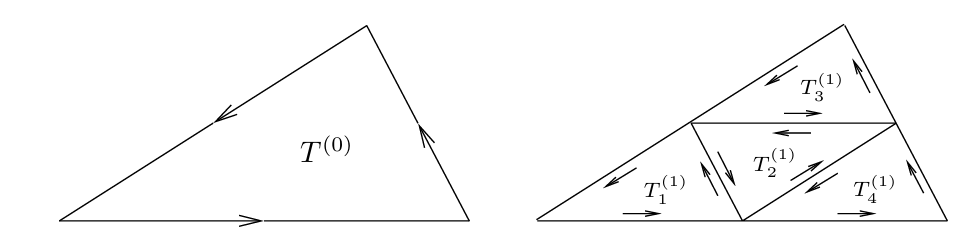
\includegraphics[width=0.5\linewidth]{Images/Goursat.png}
        \caption{Goursat's Triangle}
    \end{figure}
    (Note that $T^{(i)} = \triangle_i$ in the picture.) It is clear that 
    \[\int_{\partial \triangle} f(z)dz = \sum_{k=1}^4 \int_{\partial \triangle_k}f(z)dz.\] By the triangle inequality, 
    \[\left|\int_{\partial \triangle}f(z)dz\right| \leq \sum_{k=1}^4 \left|\int_{\partial \triangle_k}f(z)dz\right| \leq 4 \left|\int_{\partial \triangle_{(1)}}f(z)dz\right|\] We know that 
    \[d_1 = \text{diam}(\triangle_{(1)}) \leq \frac{d_0}{2} \qquad \ell_1 = \text{length}(\partial \triangle_{(1)}) \leq \frac{\ell}{2}.\]
    
    Split up $\triangle_{(1)}$ into four sub-triangles with the same process as before. We can induct on this process to find a sequence such that
    \[\triangle_{(1)}\supset \triangle_{(2)}\supset \cdots , \qquad \left|\int_{\partial \triangle}f(z)dz\right|  \leq 4^n \left|\int_{\partial \triangle_{(n)}}f(z)dz\right|, \qquad d_n \leq \frac{d_0}{2^n} \qquad \ell_n \leq \frac{\ell_0}{2^n}\] Since $\bbC$ is complete, we can use Cantor's nested set theorem to find some $z_\infty \in \bigcap \triangle_{(n)}.$ Let $\epsilon>0.$ Since $f$ is holomorphic at $z_\infty,$ we have that for $z$ close to $z_\infty,$ 
    
    if we call $R$ to be an error function such that $R(z)\to 0$ as $z\to z_{\infty},$ 
    \[f'(z_\infty) = \frac{f(z) - f(z_\infty)}{z- z_\infty} + R(z) \iff f(z)= f'(z_{\infty})(z - z_{\infty}) - R(z)(z - z_{\infty}) + f(z_{\infty}).\]
    We can use the fact that $f(z_\infty)$ and  $f'(z_\infty)(\zeta - z_0)$ are linear functions with primitives to calculate
    \begin{align*}
    \int_{\partial \triangle_{(n)}}f(z)dz &= \int_{\partial \triangle_{(n)}} [f(z_\infty) + f'(z_\infty)(z - z_\infty)] + R(z)(z- z_{\infty}) d\zeta \\
    &= \int_{\partial \triangle_{(n)}}R(z)(z - z_\infty)\,dz
    \end{align*}
    Hence, since $z$ lies on $\partial \triangle_{(n)},$ then 
    \[\left|\int_{\partial \triangle_{(n)}}f(z)dz\right| \leq \frac{\ell_0   }{2^n} \frac{d_0}{2^n}\epsilon'.\] Thus, choosing $\epsilon'= \frac{\epsilon}{d_0, \ell_0}$
    \[\left|\int_{\partial \triangle}f(z)dz\right| <\epsilon\]
\end{proof}

\begin{thm}
    (Cauchy) Suppose $O\subseteq \bbC$ is an open, convex set, and $f\in H(O).$ Then for every closed path $\gamma$ in $O,$ 
    \[\int_\gamma f(z)dz = 0\]
\end{thm}

\begin{proof}
    It suffices to show that $f$ has a primitive. Fix $z_0 \in O.$ Let $z\in O.$ Let $[z_0, z]$ be the straight line from $z_0$ to $z.$ Define
    \[F(z) = \int_{[z_0, z]}f(\zeta)d\zeta.\] To see that $F' = f,$ consider that $F(z)$ integrates from $[z_0, z],$ $F(z + h)$ integrates from $[z_0, z + h],$ and we claim that $F(z + h) - F(z)$ integrates from $[z,z + h].$ Note that if we show this, then we formed a triangle, $\triangle$. To show this, 
    consider that by Goursat,
    \[\int_{\partial \triangle} f(\zeta)d\zeta = \int_{[z_0, z]} f(\zeta)d\zeta + \int_{[z, z + h]} f(\zeta)d\zeta + \int_{[z + h, z_0]} f(\zeta)d\zeta = 0,\] and thus 
    \[\int_{[z_0, z]} f(\zeta)d\zeta + \int_{[z, z + h]} f(\zeta)d\zeta - \int_{[z_0, z + h]} f(\zeta)d\zeta = 0 \implies F(z + h)- F(z)= \int_{z, z + h}f(\zeta)d\zeta\]
    Thus, since $f$ is continuous at $z$, then for any $\epsilon>0,$ if $|\zeta - z|< \delta,$ then $|f(\zeta) - f(z)|< \epsilon.$ Take $h< \frac{1}{2}\delta,$ then 
    \begin{align*}
    F(z + h) - F(z) &= \int_{[z, z + h]}f(\zeta)d\zeta\\
        \left|\frac{F(z + h) - F(z)}{h} - f(z)\right| &= \left|\frac{1}{h}\int_{[z, z + h]}f(\zeta)d\zeta - \frac{1}{h}\int_{[z,z + h]}f(z)\right|\\
        &= \frac{1}{|h|}\left|\int_{z, z + h} f(\zeta) - f(z)d\zeta\right|\\
        &\leq \frac{1}{|h|}\text{length}(z, z + h) \max_{\zeta\in [z, z + h]}|f(\zeta) - f(z)|\\
        &= \max_{\zeta \in [z, z + h]}|f(\zeta) - f(z)|\\
        &< \epsilon
    \end{align*}
\end{proof}

\newpage
\subsection{Tuesday, Apr 22: Goursat's Theorem and the Cauchy Integral Formula}
\begin{thm}
    (Goursat) Let $O \subseteq \bbC$ is an open set and $f\in H(O \sm \{z\}),$ where $f$ is merely continuous at $z.$ Then if $\triangle \subseteq \bbC$ is closed,
    \[\int_{\triangle} f(\zeta)d\zeta = 0.\]
\end{thm}
\begin{proof}
We first sketch the proof.
    If $z \notin \triangle,$ then by Cauchy-Goursat's Theorem, we are done. Thus, assume $z\in \triangle.$ Make three triangles, $\triangle_1, \triangle_2, \triangle_3,$ where $\triangle_i \subseteq \triangle$ and $\bigcap \triangle_k = z,$ and the orientation of the triangles cancel out on the inside.  
    \begin{figure}[H]
        \centering
        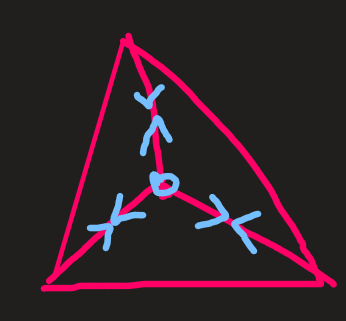
\includegraphics[width=0.25\linewidth]{Images/Goursat2.png}
        \caption{$z$ is the middle point}
    \end{figure}
    If $z_0$ is on the vertex, we can make another three triangles, as follows: 
    \begin{figure}[H]
        \centering
        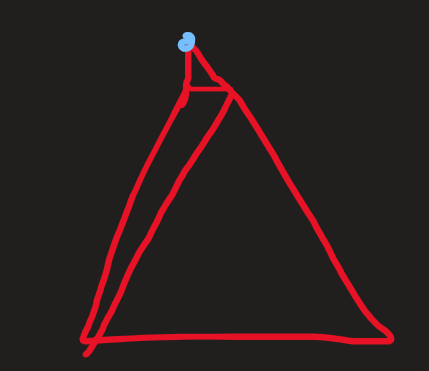
\includegraphics[width=0.25\linewidth]{Images/Gorusat3.png}
        \caption{$z_0$ is the blue point}
    \end{figure}
    We can make the top triangle as small as we wish. Thus, we can bound the line integral using Proposition 3, namely we can make it be $0.$ 
\end{proof}
\begin{thm}
(Cauchy Integral Formula)
    Suppose $O \subseteq \bbC$ is open and $\overline{D_r(z_0)} \subseteq O.$ Suppose that $f\in H(O).$ Then if $z\in D_r(z_0),$ we have that 
    \[f(z) = \frac{1}{2\pi i }\int_{C_r(z_0)}\frac{f(\zeta)}{\zeta - z}d\zeta,\] where $C_r(z_0)$ is the circle of radius $r$ centered at $z_0. $
\end{thm}
\begin{exmp}
    We have that $C_r(z_0) (\theta) = z_0 + re^{i\theta}$
\end{exmp}
\begin{proof}
    Define $F(\zeta) = \begin{cases}
        \frac{f(\zeta) - f(z)}{\zeta - z}, \quad \zeta \neq z\\
        f'(z), \qquad \;\, \zeta = z
    \end{cases}.$ It is not hard to show $F$ is continuous. For all $\zeta \neq z,$ $F$ is holomorphic. Goursat theorem tells us we can forgive $F$ for its blunder at $z,$ and thus Cauchy's Theorem, 
    \[\int_{C_r(z_0)}F(\zeta) d\zeta = 0 \implies \frac{1}{2\pi i }\int_{C_r(z_0)}F(\zeta) d\zeta.\] For small enough $r,$ we have that 
    \[\frac{1}{2\pi i }\int_{C_r(z_0)}\frac{f(\zeta) - f(z)}{\zeta - z} d\zeta = 0.\] Thus, 
    \begin{align*}
        0 & =\frac{1}{2\pi i }\int_{C_r(z_0)}\frac{f(\zeta) - f(z)}{\zeta - z} d\zeta\\
        &= \frac{1}{2\pi i} \int_{C_r(z_0)}\frac{f(\zeta)}{\zeta - z} d\zeta - \frac{1}{2\pi i} \int_{C_r(z_0)}\frac{f(z)}{\zeta - z} d\zeta\\
        &= \frac{1}{2\pi i} \int_{C_r(z_0)}\frac{f(\zeta)}{\zeta - z} d\zeta - \frac{f(z)}{2\pi i} \int_{C_r(z_0)}\frac{1}{\zeta - z} d\zeta\\
        &= \frac{1}{2\pi i} \int_{C_r(z_0)}\frac{f(\zeta)}{\zeta - z} d\zeta - f(z)\Ind_{C_r(z_0)}(z)\\
        &=\frac{1}{2\pi i} \int_{C_r(z_0)}\frac{f(\zeta)}{\zeta - z} d\zeta - f(z)
    \end{align*}
\end{proof}
\begin{rem}
    With the same assumptions as the above, we have that 
    \begin{align*}
    f(z) &= \frac{1}{2\pi i }\int_{C_r(z_0)}\frac{f(\zeta)}{\zeta - z}d\zeta\\
    &= \frac{1}{2\pi i }\int_{C_r(z_0)}\frac{f(\zeta)}{\zeta - z_0 - (z - z_0)}d\zeta\\
    &= \frac{1}{2\pi i }\int_{C_r(z_0)}\frac{f(\zeta)}{(\zeta - z_0)} \frac{1}{1 - \frac{z-z_0}{\zeta - z_0}}d\zeta \\
    &= \frac{1}{2\pi i }\int_{C_r(z_0)}\frac{f(\zeta)}{(\zeta - z_0)} \frac{1}{1 - a}d\zeta\\
    &=\frac{1}{2\pi i }\int_{C_r(z_0)}\frac{f(\zeta)}{(\zeta - z_0)} \sum_{n=0}^\infty \frac{(z - z_0)^n}{(\zeta - z_0)^n}d\zeta
    \end{align*}
Recall the Weierstrass M-test. If $G_N(s) = \sum_{k=1}^N g_k(s),$ where $|g_k(s)| \leq M_k$ for all $k,$ and $\sum_{k=1}^\infty M_k < \infty,$ then $G_n$ converges uniformly. We have that 
\[\left|G_n(s) - G_m(s)\right|  = |\sum_{m+1}^n g_k| \leq |\sum_{m+1}^n |g_k| \leq \sum_{m+1}^n M_k < \epsilon,\] and thus $G_n$ is a Cauchy sequence of real numbers. Thus, by completeness, we have that $\|G(s) - G_n(s)\|_{\sup (s)} < \epsilon.$ Thus, since the $F_N$ converge uniformly to $F_\infty,$ then we have that 
\[\lim_{n\to \infty} \int F_n = \int F,\] and thus 
\begin{align*}
    \frac{1}{2\pi i }\int_{C_r(z_0)}\frac{f(\zeta)}{(\zeta - z_0)} \sum_{n=0}^\infty \frac{(z - z_0)^n}{(\zeta - z_0)^n}d\zeta &= \lim_{N \to \infty} \frac{1}{2\pi i }\int_{C_r(z_0)}\frac{f(\zeta)}{(\zeta - z_0)} \sum_{n=0}^N\frac{(z - z_0)^n}{(\zeta - z_0)^n}d\zeta\\
    &= \lim_{N\to \infty} \sum_{n=0}^N\frac{1}{2\pi i }\int_{C_r(z_0)}\frac{f(\zeta)}{(\zeta - z_0)}  \frac{(z - z_0)^n}{(\zeta - z_0)^n}d\zeta\\
    &= \sum_{n=0}^\infty \left[\frac{1}{2\pi i }\int_{C_r(z_0)}\frac{f(\zeta)}{(\zeta - z_0)^{n+1}}\right]  (z - z_0)^nd\zeta
\end{align*}
Thus, $f(z)$ is equal to a convergent power series inside of a disk. In particular, $f(z)$ is infinitely differentiable since power series are infinitely differentiable!!!!! (See Corollary 1).
\end{rem}
We summarize this remark with the following theorem.
\begin{thm}
    Suppose $\overline{D_r(z_0)} \subseteq O,$ where $O$ is open and $f\in H(O).$ Then $f$ is infinitely differentiable. 
\end{thm}
\begin{rem}
    Consider the special case of the Cauchy integral formula:
    \begin{align*}
    f(z_0) &= \frac{1}{2\pi i}\int_{C_r(z_0)} \frac{f(\zeta)}{\zeta - z_0}d\zeta\\
    &= \frac{1}{2\pi i} \int_0^{2\pi} \frac{f(z_0 + re^{i\theta})}{z_0 + re^{i\theta} - z_0}ir e^{i \theta}d\theta\\
    &= \frac{1}{2\pi i} \int_0^{2\pi} f(z_0 + re^{i\theta})d\theta
    \end{align*}
    We recognize this as the mean value property from PSET 1.
\end{rem}

\begin{cor}
    
\end{cor}
\begin{proof}
    Since $f(z) = \sum_{n=0}^\infty a_n(z - z_0)^n,$ where $a_n = \frac{1}{2\pi i} \int_{C_r(z_0)} \frac{f(\zeta)}{(\zeta - z_0)^{n+1}}d\zeta.$ By a previous theorem, we know also that 
    \[a_n = \frac{f^{(n)}(z_0)}{n!}\]
\end{proof}

\newpage
\subsection{Thursday, Apr 24: Louisville's Theorem}

Today he proved everything he did last class again, so you can look at last classes note's for that. 
\begin{thm}
    (Louisville) If $f \in H(\bbC)$ and $|f(z)| \leq M$ for all $z\in \bbC,$ then $f$ is constant.
\end{thm}
\begin{proof}
By Corollary $2$ in the previous class, we have that 
\[f'(z_0) = \frac{1}{2\pi i} \int_{C_r(z_0)}\frac{f(\zeta)}{(\zeta - z_0)^2}d\zeta,\] and thus 
\[|f'(z_0)| \leq  |\frac{1}{2\pi i}|\text{length}(C_r(z_0)) \max_{\zeta \in C_z(r)} \left|\frac{f(\zeta)}{(\zeta - z_0)^2}\right| \leq \frac{1}{2\pi }2\pi r  \frac{M}{r^2} = \frac{M}{r }.\] But since $f$ is holomorphic over all of $\bbC,$ we can take $r \to \infty,$ and thus $|f'(z_0)| \leq 0,$ and so because $z_0$ was arbitrary in $\bbC,$ $f$ is constant.
\end{proof}

\begin{rem}
    Let $P$ be a non-constant polynomial Suppose that $P(z) \neq 0$ for any $z,$ then as $z\to \infty,$ 
    \[|P(z)| \to \infty.\] Then $\frac{1}{|P(z)|} \to 0$ and since $\frac{1}{P(z)}$ is bounded and holomorphic, then it is constant, and thus $P(z)$ is constant. Thus, we have the fundamental theorem of algebra.
\end{rem}

\newpage
\subsection{Tuesday, Apr 29: Fundamental Theorem of Algebra}
\begin{rem}
    Recall that 
    \[f(z) = \frac{1}{2\pi i }\int_{C_r(z_0)}\frac{f(\zeta)}{\zeta - z}d\zeta = \sum_{n=0}^\infty a_n (z- z_0)^n.\] Then
    \[a_n = \frac{1}{2\pi i}\int_{C_{r}(z_0)}\frac{f(\zeta)}{(\zeta - z_0)^{n+1}}d\zeta = \frac{1}{n!}f^{(n)}(z_0)\]
Thus, for $n = 1,$ we have that 
\[f'(z_0) = \frac{1}{2\pi i} \int_{C_r(z_0)}\frac{f(\zeta)}{(\zeta- z_0)^2}d\zeta,\] and so the rate of change is dependent on the size of the function, hence why Louisville's theorem makes sense.
\end{rem}
\begin{thm}
    Suppose $f$ is an entire function that is bounded. Then $f$ is constant.
\end{thm}
\begin{proof}
Since $f$ is bounded, we have that $|f(\zeta)| \leq M$ for all $\zeta\in M.$
    By the remark above, we know that 
    \begin{align*}
        |f
        '(z_0)| &\leq \frac{1}{2\pi }\big|\text{arclength}\big[C_r(z_0)\big]\big| \max_{\zeta \in C_r(z_0)} |\frac{f(\zeta)}{(\zeta - z_0)^2}|\\
        &= \frac{1}{2\pi }2\pi r   \max_{\zeta \in C_r(z_0)} \frac{|f(\zeta)|}{(\zeta - z_0)^2}\\
        &\leq \frac{M}{2\pi }2\pi  r  \max_{\zeta \in C_r(z_0)} \frac{1}{(\zeta - z_0)^2}\\
        &= \frac{M}{2\pi }2\pi r \frac{1}{r^2}\\
        &= \frac{M}{r}
    \end{align*}
    But $f \in H(O),$ and so we can let $r\to \infty,$ implying that $f'(z_0) = 0$ for all $z_0 \in \bbC.$
\end{proof}

\begin{thm}
    (Fundamental Theorem of Algebra) If $P(z)$ is a polynomial with degree of more than zero, then $P(z_0) = 0$ for some $z_0 \in \bbC.$
\end{thm}
\begin{proof}
    Suppose $P(z) \neq 0$ for all $z \in \bbC.$ Let 
    \[f(z) = \frac{1}{P(z)}.\] Note that $f \in H(\bbC).$ 

    Note that 
    \[|P(z)| = |a_nz^n + a_{n-1}z^{n-1} + \cdots + a_0| = |z^n|\left|(a_n + \frac{a_{n-1}}{z} + \cdots + \frac{a_0}{z^n})\right| \xrightarrow[z\to \infty]{} \infty\] Thus,, we have that 
    \[f(z) = \frac{1}{|P(z)|}\to 0.\] Thus, there exists some closed $D_r(0)$ such that for all $z\notin D_r(0),$ we have that $|f(z)| < \epsilon.$ Since $f$ is continuous on the compact disk, we have that $f$ is bounded by the extreme value theorem. Thus, $|f(z)| < M$ for all $z\in \bbC.$ Thus, by Louisville's theorem, $f(z) = \frac{1}{P(z)}$ is constant, and thus $P(z)$ is constant, which is a contradiction.
\end{proof}

\begin{defn}
Let $f\in H(O)$ and $z\in O.$ The \textbf{Laurent Series} of $f$ is the series
    \[f(z) = \sum_{n=-\infty}^\infty a_n (z - z_0)^n\]
\end{defn}
\begin{exmp}
    Consider $C = D_1(0)\sm \{0\}$ to be the punctured disk and consider $f(z) = \frac{1}{z}.$
\end{exmp}
\begin{defn}
Let $\gamma:[0,1] \to O$ be a path.
    We define a \textbf{homotopy} in $O \subset \bbC$ to be a function $\Gamma(t,s) : [0,1] \times [0,1] \to O$ such that $\gamma_s(t) = \Gamma(t,s)$ and
    \begin{enumerate}
        \item $\Gamma$ is continuous from $[0,1]\times [0,1].$
        \item For all $s\in [0,1],$ $\Gamma(0,s) = \gamma_s(0) = z_1$ and $\Gamma(1,s) = \gamma_s(1) = z_2.$
        \item For each $s\in [0,1],$ $\gamma_s(t)$ is a path and for each $t\in [0,1],$ the map $s\mapsto \gamma_s(t)$ is piecewise continuously differentiable as a function of $s.$
    \end{enumerate}
\end{defn}

We will next show the invariancy of line integrals about homotopies, and use that for the Laurent series. 


\newpage
\subsection{Tuesday, May 6: Homotopic Defomations}
Let $A$ be an annulus around $z_0.$ Clearly, if $f \in H(A),$ then we cannot express $f(z)$ as a convergent power series, since then $f$ would be holomorphic within the disk. The following few lectures will talk about how useful Laurent series are in expressing functions like this. First we discuss homotopies in detail.

\begin{defn}
    A \textbf{homotopic deformation} of a path $\gamma_0$ connecting $z_1$ to $z_2$ to a path $\gamma_1$ also connecting $z_1$ to $z_2$ is a function $\Gamma(t,s): [0,1]^2 \to O$ such that     \begin{enumerate}
        \item $\Gamma$ is continuous from $[0,1]\times [0,1].$
        \item For all $s\in [0,1],$ $\Gamma(0,s) = \gamma_s(0) = z_1$ and $\Gamma(1,s) = \gamma_s(1) = z_2.$
        \item For each $s\in [0,1],$ $\gamma_s(t)$ is a path and for each $t\in [0,1],$ the map $s\mapsto \gamma_s(t)$ is piecewise continuously differentiable as a function of $s.$
    \end{enumerate}
\end{defn}
Intuitively, $s$ measures how far along the deformation has gone on, the line from bottom to top is a path, and all these paths are continuous. 
\begin{rem}
    Since $\Gamma([0,1]\times [0,1])$ is compact since $\Gamma$ is continuous, and since $O^c$ is closed, then for every $w\in O^c,$ there exists some $\epsilon>0$ such that 
    \[|\Gamma(s,t) - w| = |\gamma_s(t), w| \geq \epsilon >0.\]
    Equivalently, 
    \[D_{\frac{\epsilon}{2}}(\Gamma(s_0, t_0)) \subseteq O, \quad \forall (s_0, t_0) \in [0,1]^2\]

    Moreover, since $\Gamma$ is continuous and the domain is compact, then $\Gamma$ is uniformly convergent. Thus, take $\delta>0$ such that if $d((s_1, t_1), (s_2, t_2))< \delta,$ then $d(\Gamma(s_1, t_1), \Gamma(s_2, t_2)) < \frac{\epsilon}{2}.$ 

    Partition $[0,1]^2$ into squares, $S_k,$ of equal diameter which is less that $\delta.$ Thus, $\Gamma(S_k)\subseteq D_{\frac{\epsilon}{2}}(z)$ for some $z \in O.$ Consider the path, $\gamma_{S_k}$,  formed by traversing each $S_k$  by the four time intervals (the sides of the square). Then $\gamma_{S_k}\subseteq D_{\frac{\epsilon}{2}}(z),$ and so by Cauchy's theorem, since $f\in H(O),$ we have that 
    \[\int_{\gamma_{S_k}}f(z)\, dz = 0\] Then 
    \[\sum_k \int_{\gamma_{S_k}}f(z)\, dz = 0,\] but since we can make it so the orientations cancel each other out, then you end up with the path over the boundary of $[0,1]^2.$ Since the left and right vertical boundary lines are simply constant $z_1$ and $z_2,$ then
    \[ \int_{\gamma_0}f(z)\, dz - \int_{\gamma_1} f(z)\, dz= \sum_k \int_{\gamma_{S_k}}f(z)\, dz = 0\] and so
    \[\int_{\gamma_0} f(z)\, dz = \int_{\gamma_1} f(z)\,dz\]
\end{rem}
\begin{thm}
    Let $O\subset \bbC$ be open, and suppose that $\gamma_1$ and $\gamma_2$ are homotopically deformable paths. Then if $f\in H(O),$ 
    \[\int_{\gamma_0} f(z)\, dz = \int_{\gamma_1} f(z)\,dz\]
\end{thm}
\begin{proof}
    The proof follows from Remark 17
\end{proof}

\begin{defn}
    We say that a region $O \subset \bbC$ is \textbf{simply connected} if every closed path $\gamma$ is homotopically  deformable to a point path
\end{defn}

\begin{thm}
    Suppose $O\subseteq \bbC$ is simply connected and $f\in H(O).$ Then for any path $\gamma$ in $O,$ 
    \[\int_\gamma f(z)\, dz = 0\]
\end{thm}
\begin{proof}
    We can apply Theorem 18 to establish the equivalence between a point path and our path $\gamma.$
\end{proof}

\begin{thm}
    Let $A$ be an annulus. Let $f \in H(A)$ and fix $z\in A$ between $\gamma_i$ and $\gamma_0,$ where $\gamma_i$ is a circle around the inner disk of $A$ and $\gamma_0$ is a large circle around $\gamma_i.$ Then 
    \[\int_{\gamma_i}f(z)\, dz = \int_{\gamma_0}f(z)\, dz.\]
\end{thm}
\begin{proof}
    Consider the function 
    \[F(\zeta) = \begin{cases}
        \frac{f(\zeta) - f(z)}{\zeta - z}, \qquad \zeta \neq z\\
        f'(z)
    \end{cases}.\] Then $F$ is holomorphic and so 
    \[\frac{1}{2\pi i}\int_{\gamma_i}F(\zeta)d\zeta = \frac{1}{2\pi i}\int_{\gamma_i}\frac{f(\zeta)}{\zeta - z}\,d\zeta - f(z) \int_{\gamma_i} \frac{d\zeta}{\zeta - z} = \frac{1}{2\pi i}\int_{\gamma_0}\frac{f(\zeta)}{\zeta - z}\,d\zeta - f(z) \int_{\gamma_0} \frac{d\zeta}{\zeta - z}\] But clearly, 
    \begin{align*}
        \frac{1}{2\pi i}\int_{\gamma_i}\frac{f(\zeta)}{\zeta - z}\,d\zeta &= \frac{1}{2\pi i}\int_{\gamma_i}\frac{f(\zeta)}{\zeta - z}\,d\zeta - f(z) \int_{\gamma_i} \frac{d\zeta}{\zeta - z}\\ &= \frac{1}{2\pi i}\int_{\gamma_0}\frac{f(\zeta)}{\zeta - z}\,d\zeta - f(z) \int_{\gamma_0} \frac{d\zeta}{\zeta - z}\\
        &= \frac{1}{2\pi i}\int_{\gamma_0}\frac{f(\zeta)}{\zeta - z}\,d\zeta - f(z) 
    \end{align*} and thus 
    \[f(z) = \frac{1}{2\pi i}\int_{\gamma_0} \frac{f(\zeta)}{\zeta - z}\, d\zeta + \frac{1}{2\pi i}\int_{\gamma_i} \frac{f(\zeta)}{z - \zeta}d\zeta\]
\end{proof}


\newpage
\subsection{Thursday, May 8: Riemann's Theorem and the Weierstrass Casserati Theorem}
We begin by redoing the derivation of the formula for the Laurent series from last class. 
\[\begin{tikzpicture}[scale=1]
      % define center
      \coordinate (O) at (0,0);
      % shade the annulus
      \fill[blue!10, even odd rule]
        (O) circle (2cm)
        (O) circle (1cm);

      % draw outer circle gamma_0 with arrow
      \draw[thick, ->] 
        (2,0) arc (0:360:2cm) 
        node[midway, right] {$\gamma_0$};

      % draw inner circle gamma_i with arrow (opposite orientation if desired)
      \draw[thick, ->] 
        (1,0) arc (0:360:1cm)
        node[midway, left] {$\gamma_i$};

      % mark and label the center z_0
      \fill (O) circle (1.5pt) node[below left] {$z_0$};

      % place and label the point z
      \coordinate (Z) at (1.25,0.7);
      \fill (Z) circle (1.5pt) node[above right] {$z$};
    \end{tikzpicture}\]
\begin{figure}[H]
    \centering
    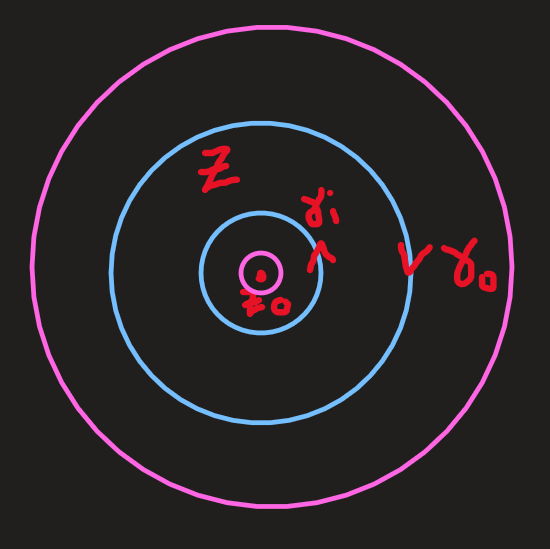
\includegraphics[width=0.5\linewidth]{Images/anus.png}
    \caption{The Annulus and the Paths}
\end{figure}
Call 
\[F(\zeta) = \begin{cases}
    \frac{f(\zeta) - z }{\zeta - z}, \quad \zeta\neq z\\
    f'(z), \quad \zeta = z
\end{cases}\] to be a holomorphic function. While $\gamma_0$ and $\gamma_1$ are not homotopically equivalent, then can be made that by a single line going out and in of the inner and out circle, but those line integrals cancel out. Thus, by Theorem 18, 
\[\int_{\gamma_1}F(\zeta)\,d\zeta = \int_{\gamma_0}F(\zeta)\,d\zeta\]
\[\frac{1}{2\pi i}\int_{\gamma_1}F(\zeta)\,d\zeta =\frac{1}{2\pi i} \int_{\gamma_0}F(\zeta)\,d\zeta\]
\[ \frac{1}{2\pi i}\int_{\gamma_i}\frac{f(\zeta)}{\zeta - z}\,d\zeta - f(z) \int_{\gamma_i} \frac{d\zeta}{\zeta - z} = \frac{1}{2\pi i}\int_{\gamma_0}\frac{f(\zeta)}{\zeta - z}\,d\zeta - f(z) \int_{\gamma_0} \frac{d\zeta}{\zeta - z}\]
The winding number of the left side is $0,$ while the winding number of the right side is $1.$ Hence, 
\[\frac{1}{2\pi i}\int_{\gamma_i}\frac{f(\zeta)}{\zeta - z}\,d\zeta  = \frac{1}{2\pi i}\int_{\gamma_0}\frac{f(\zeta)}{\zeta - z}\,d\zeta - f(z)\]
And we then compute:
\begin{align*}
    f(z) &= \frac{1}{2\pi i}\int_{\gamma_0}\frac{f(\zeta)}{\zeta - z}\,d\zeta  - \frac{1}{2\pi i}\int_{\gamma_i}\frac{f(\zeta)}{\zeta - z}\,d\zeta\\
    &= \frac{1}{2\pi i}\int_{\gamma_0}\frac{f(\zeta)}{\zeta - z}\,d\zeta  + \frac{1}{2\pi i}\int_{\gamma_i}\frac{f(\zeta)}{z - \zeta}\,d\zeta\\
    &= \frac{1}{2\pi i}\int_{\gamma_0}\frac{f(\zeta)}{(\zeta - z_0) - (z - z_0)}\,d\zeta  + \frac{1}{2\pi i}\int_{\gamma_i}\frac{f(\zeta)}{(z -z_0) - (\zeta -  z_0)}\,d\zeta\\
    &= \frac{1}{2\pi i}\int_{\gamma_0}\frac{1}{1 - \frac{(z - z_0)}{(\zeta - z_0)}} \frac{f(\zeta)}{\zeta - z_0}\,d\zeta  + \frac{1}{2\pi i}\int_{\gamma_i}\frac{1}{1 - \frac{\zeta - z_0}{z - z_0}} \frac{f(\zeta)}{z - z_0}\,d\zeta\\
    &=  \frac{1}{2\pi i}\int_{\gamma_0}\sum_{n=0}^\infty \left(\frac{z - z_0}{\zeta - z_0}\right)^n \frac{f(\zeta)}{\zeta - z_0}\,d\zeta  + \frac{1}{2\pi i}\int_{\gamma_i}\sum_{n=0}^\infty \left(\frac{\zeta - z_0}{z - z_0}\right)^n\frac{f(\zeta)}{z - z_0}\,d\zeta\\
    &= \sum_{n=0}^\infty \frac{1}{2\pi i}\int_{\gamma_0} \frac{f(\zeta)}{(\zeta - z_0)^{n+1}} (z - z_0)^n + \sum_{n=0}^\infty \frac{1}{2\pi i}\int_{\gamma_i} (\zeta - z_0)^n f(\zeta)(z - z_0)^{-(n+1)}\\
    &= \sum_{n=0}^\infty \frac{1}{2\pi i}\int_{\gamma_0} \frac{f(\zeta)}{(\zeta - z_0)^{n+1}} (z - z_0)^n + \sum_{n=-\infty}^{-1} \frac{1}{2\pi i}\int_{\gamma_i} (\zeta - z_0)^{-(n+1)}f(\zeta)(z - z_0)^{n}\\
    &= \sum_{n=0}^\infty \frac{1}{2\pi i}\int_{\gamma_0} \frac{f(\zeta)}{(\zeta - z_0)^{n+1}} (z - z_0)^n + \sum_{n=-\infty}^{-1} \frac{1}{2\pi i}\int_{\gamma_i} \frac{f(\zeta)}{(\zeta - z_0)^{-(n+1)}}(z - z_0)^{n}\\
    &= \sum_{n=0}^\infty \frac{1}{2\pi i}\int_{\gamma} \frac{f(\zeta)}{(\zeta - z_0)^{n+1}} (z - z_0)^n + \sum_{-\infty}^{-1} \frac{1}{2\pi i}\int_{\gamma} \frac{f(\zeta)}{(\zeta - z_0)^{(n+1)}}(z - z_0)^{n}\\
    &= \sum_{n=-\infty}^{\infty} \frac{1}{2\pi i}\int_{\gamma} \frac{f(\zeta)}{(\zeta - z_0)^{n+1}}(z - z_0)^{n}
\end{align*}

\begin{thm}
    (Riemann) Suppose $f \in H(D_{\epsilon}(z_0) \sm \{z_0\})$ and $|f(z)| \leq M$ for all $z \in D_{\epsilon}(z_0) \sm \{z_0\}.$ Then we can define $f(z_0)$ such that $f \in H(D_\epsilon(z_0)).$
\end{thm}
\begin{proof}
    Let $r>0,$ and let $\gamma_r$ be a circle of radius $r$ about $z_0.$ 
    \[|a_{-n}| = \left|\frac{1}{2\pi i}\int_{\gamma_r} f(\zeta)(\zeta - z_0)^n\right| \leq r M r ^n = Mr^{n+1}\] Thus, $a_{-n} = 0$ for any $n >0.$ Thus, as $r \to 0,$ we have that $f(z_0)$ is an absolutely convergent power series.
\end{proof}

\begin{thm}
    (Weierstrass-Casserati) Suppose $f\in H(D_\epsilon(z_0)\sm \{z_0\}).$ Then either:
    \begin{enumerate}
        \item $f$ has a removable singularity at $z_0;$
        \item $f$ has a pole at $z_0,$ i.e, 
        \[\lim_{z\to z_0}|f(z)| = \infty;\]
        \item $f$ has an essential isolated singularity if it is neither (a) or (b). Then the image of $f$ when we consider the domain $D_\delta(z_0) \sm \{z_0\}$ for $0 < \delta < \epsilon$ is dense in $\bbC.$
    \end{enumerate}
\end{thm}

\begin{proof}
    If $f$ has no negative terms in the Laurent series, then $f$ can be expressed as a convergent power series. If $f$ is bounded, then it clearly a removable singularity. If $f$ has at most finitely many negative powers in the Laurent expansion, then for $z$ such that $0 < |z - z_0| < \epsilon,$ take $n_k$ to be the highest negative power
    \begin{align*}
    |f(z)| &= \frac{a_{n_k}}{(z - z_0)^{n_k}} + \frac{a_{n_{k=1}}}{(z - z_0)^{n_{k-1}}} + \cdots+ \sum_{n=0}^\infty a_n (z - z_0)^n\\ &=  \frac{1}{(z - z_0)^{n_k}}\left(a_{n_k}+ a_{n_{k-1}}(z - z_0)^{m_k} + \cdots + a_{n_1}(z - z_0)^{m_1} \right) + \sum_{n=0}^\infty a_n (z - z_0)^n \\
    &\to \infty
    \end{align*}
\end{proof}

\newpage
\subsection{Tuesday, May 13: Poles and Introducing the Residue Theorem}

Continuing the proof from last class, where we were dealing with essential isolated singularities. Before we do so, consider the following example:
\begin{exmp}
    Consider the function $f(z) = e^\frac{1}{z}.$ Then our puncture disk is $\bbC\sm \{0\}.$ The expansion is
    \[e^{\frac{1}{z}} = 1 + \frac{1}{1!}\frac{1}{z} + \frac{1}{2!}(\frac{1}{z})^2 + \cdots\] Clearly, as $z\to 0,$ the function blows up, and so we can see why this essential singularity theorem could be true.
\end{exmp}
\begin{proof}
Suppose now $f$ has infinitely many negative powers in the Laurent expansion of $z_0$. But suppose, for the sake of contradiction, that there exists some $\epsilon>0$ such that the value set of $f(z)$ for $z\in D_\epsilon(z)$ that is not dense in $\bbC.$ Thus, there is some open disk in $\bbC$ that contains no such $f(z).$ Thus, $f(z) \notin D_\delta(\alpha)$ for some $\delta>0$ and $\alpha \in \bbC.$ Consider now 
\[g(z) = \frac{1}{f(z) - \alpha}\] for $D_\epsilon(z_0)\sm \{z_0\}.$ We know that $g$ is bounded since the denominator is bounded below by $\delta.$ Hence, by Riemann's Theorem (21), we can define $g(z_0)$ such that $g(z_0) \in H(D_\epsilon(z_0)).$ If $g(z_0) \neq 0,$ then $f(z) - \alpha$ is holomorphic at $z_0,$ contradicting the fact that $z_0$ is an essential singularity. If $g(z_0) = 0,$ then $f$ has a pole at $z_0,$ another contradiction.
\end{proof}

\begin{defn}
Suppose $f\in H(D_\epsilon(z_0))$ for some $z_0 \in \bbC.$
    We say that $f$ has a \textbf{zero of order $N$} at $z_0$ if 
    \[f(z) = \sum_{n = N}a_n (z - z_0)^n\]
\end{defn}
\begin{rem}
    Clearly, 
    \[f(z_0) = f'(z_0) = \cdots = f^{(N-1)}(z_0)  =0\] and $f^{(N)}(z_0) \neq 0.$
\end{rem}


\begin{defn}
    Suppose $f \in H(D_\epsilon(z_0)\sm \{z_0\})$ and $f$ has a \textbf{pole of at $z_0 $ of order $N$} if the negative powers of the Laurent series are both finite and the smallest negative power is of order $N.$
\end{defn}

\begin{defn}
    Let $O\subseteq \bbC$ be an open set and suppose $f: O\sm S \to \bbC,$ where $S$ has no limit points in $O$ and $f \in H(O \sm S).$ If at each point of $S,$ $f$ has either a removable singularity or a pole, then $f$ is \textbf{meromorphic.}
\end{defn}

\begin{rem}
    In this class, $S = \{z_0, z_1, \dots, z_n\}$ is finite.
\end{rem}
\begin{defn}
    Suppose $f$ has an isolated singularity at $z_0,$ and the Laurent expansion at $z_0$ is 
    \[f(z_0) = \sum_{-\infty}^\infty a_n (z - z_0)^n,\] then the \textbf{residue} of $f$ at $z_0$ is 
    \[\Res_{z_0}{f} = a_{-1}\]
\end{defn}

\begin{thm}
(Residue Theorem)
Let $f$ be meromorphic in a simply connected region $O$ with poles at $z_0, \dots, z_N.$ Let $\gamma$ be any closed path in $O$ not passing through any of the poles. Then 
\[\int_\gamma f(z)\,dz = 2\pi i \sum_{k=0}^N \Ind_\gamma(z_k) \Res_{z_k}f\]
\end{thm}


\newpage
\subsection{Thursday, May 15: The Residue Theorem}
\begin{thm} (Residue Theorem)
    Suppose $O$ is a simply connected region and $f$ is meromorphic in $O.$  Let $\gamma$ be a closed path not passing through any of the $n$ poles. Then 
    \[\int_\gamma f(z)\,dz = 2\pi i \sum_{k = 1}^n\Ind_\gamma (z_k)\Res_{z_k}(f)\]
\end{thm}
\begin{proof}
    If $f$ has a pole at $z_k,$ then by the Caseratti-Weierstrass theorem,
    \[f(z) = \sum_{j=1}^N \frac{a_j}{(z - z_k)^j} + \text{power series in $(z-z_k)$}.\] Let 
    \[P_k = \sum_{j=1}^N\frac{a_j}{(z - z_k)^j}\] be the principal part of the Laurent expansion.
    
    Thus, there is some $r_k<0$ such that if $z \in D_{r_k}(z_k),$ then $z$ is not a residual of $f.$ We claim that 
    \[f(z) - \sum_{k=1}^n P_k(z):= g(z)\in H(O).\] Consider $z_1.$ We claim that $f(z) - P_1(z)$ has a removable singularity at $z_1.$ One can see this because at $D_1(z_1),$ $f(z) - P_1(z)$ can be expressed as a power series with a removable singularity at $z_1.$ Note that $\sum_{k=2}^n P_k(z)$ does not interfere with this because of how we defined $r_1.$ Thus, $g(z)\in H(O)$ by Riemann's theorem. Hence, we use Cauchy's theorem
    \begin{align*}
    \int_\gamma f(z)\,dz &= \int_\gamma (f(z) - \sum P_k(z))\,dx + \int_\gamma P_k(z) \,dz\\ &= \int_\gamma \sum P_k(z) \,dz \\
    &= \sum_{k=1}^n \int_\gamma P_k(z)\,dz\\
    &= 2\pi i \sum_{k=1}^n \frac{1}{2\pi i}\int_\gamma \sum_{j=1}^{N_k} \frac{a_j}{(z - z_k)^j}\,dz\\
    &= 2\pi i \sum_{k=1}^n \sum_{j=1}^{N_k}\frac{a_j}{2\pi i}\int_\gamma \sum_{j=1}^{N_k} \frac{1}{(z - z_k)^j}\,dz\\
    &= 2\pi i \sum_{k=1}^n a_1^{(k)}\frac{1}{2\pi i}\int_\gamma\frac{1}{(z - z_k)}\,dz\\
    &=2\pi i \sum_{k=1}^n \frac{1}{2\pi i} \Res_{z_k}(f) \Ind_\gamma(z_k)
    \end{align*}
    
\end{proof}

\begin{exmp}
    Consider some function $f(z)$ with poles at $n\pi$ on the real axis, where $n \in \bbZ.$ Let $R>0$ such that $|n \pi |< R$ for all $n \in \bbZ.$ The consider the disk $D_R(0).$ We want this function $f(z)$ have residuals such that 
    \[\Res_{n\pi}(f) = \frac{1}{(n\pi )^2}.\] Consider now $\sin^{-1} z.$ The Laurent expansion about $0$ is 
    \[\frac{1}{\sin z} = \frac{1}{z - \frac{z^3}{3!} + \frac{z^5}{5!} + \cdots } = \frac{1}{z}\frac{1}{1 - \frac{z^2}{3!} + \frac{z^4}{5!} + \cdots}\] Near $z = 0,$ the second term is holomorphic, and thus it has a power series. Thus, 
    \[\frac{1}{\sin z} = \frac{1}{z} (a_0 + a_1z + a_2z^2 + \cdots).\] It suffices to find $a_0,$ which is clearly $1.$ Now consider 
    \[\Res_{n \pi} (\frac{1}{z^2(\sin z)})\] We have that about $n\pi,$
    \[(\frac{1}{z^2(\sin z)})=\frac{1}{z^2}\left[ \frac{1}{z - n\pi} + \text{ power series}\right]\] But $\frac{1}{z^2}$ is perfectly holomorphic about $n\pi$ for $n \neq0,$ and so it is analytic, and thus 
    \[\frac{1}{z^2(\sin z)} = (b_0 + b_1(z- n\pi)+ \cdots)\left[\frac{1}{z - n\pi} + \text {power series}\right]\] so it suffices to find $b_0,$ which is clearly $\frac{1}{(n\pi)^2}.$ Observe that as $z\to \infty,$
    \[\left|\frac{\cos z}{\sin z}\right| = \left|\frac{e^{iz}+ e^{-iz}}{e^{iz} - e^{-iz}}\right|\to 1.\] 
\end{exmp}
\begin{thm}
    \[\sum_{n=1}^\infty \frac{1}{n^2} = \frac{\pi^2}{6}\]
\end{thm}
\begin{proof}
    We claim that $\cot z$ is $\pi$ periodic. Consider that 
    \begin{align*}
        \cot z &= \frac{\cos z}{\sin z}\\
        &= \frac{\frac{e^{iz} + e^{-iz}}{ 2}}{\frac{e^{iz} - e^{-iz}}{2i}}\\
        &= i\frac{e^{i(w + \pi) + e^{-i(w + \pi)}}}{e^{i(w + \pi)} - e^{i(w + \pi)}}\\
        &= i\frac{e^{i(w)e^\pi + e^{-i(w)e^\pi}}}{e^{i(w)}e^\pi - e^{i(w)}e^\pi}\\
        &= \cot z
    \end{align*}
    We now claim that $\cot z \frac{1}{z^2}$ has a pole exactly at $n\pi$ for $n \in \bbZ.$ We can expand $\cot z$ at $0$ by 
    \begin{align*}
        \cot z &= \frac{\cos z}{\sin z}\\
        &= \frac{1 - \frac{z^2}{2!} + \frac{z^4}{4!} + \cdots}{z - \frac{z^3}{3!} + \frac{z^5}{5!} + \cdots }\\
        &= \frac{1}{z}\left[\frac{1 - \frac{z^2}{2!} + \frac{z^4}{4!} + \cdots}{1 - \frac{z^2}{3!} + \frac{z^4}{5!} + \cdots} \right]\\
        &= \frac{1}{z}(a_0 + a_1 z + \cdots)
    \end{align*}
    And so 
    \[\Rez_0 \cot(z) = a_0= 1\]

    Now consider for $n\pi \neq 0,$
    \begin{align*}
        \frac{1}{z^2} \cot z
        &= \frac{1}{z^2}\left[\frac{1}{z - n\pi} + \text{power series}\right]\\
    \end{align*}
    so it suffices to find $a_1.$ We will find next class that $a_1 = \frac{1}{n^2 \pi^2}.$
\end{proof}

\newpage
\subsection{Tuesday, May 20: $\sum \frac{1}{n^2}$}
Final: Thursday, May 29. 10am. Ryerson 358. Continuing from the previous class:
\begin{proof}
    We have shown that $\cot z$ is $\pi-$periodic and that it has poles at exactly multiples of $\pi$ and that $\Res_{n\pi} \cot z = 1.$ We also showed that $\Res_{n\pi}(\frac{\cot z}{z^2}) = \frac{1}{n^2 \pi^2}$ for $n \neq 0.$ It remains to show that if we remove $\mathcal{D} = \{D_{r}(n\pi)\}_{n \in \bbZ}$ for $r$ small, then $\frac{\cot z}{z^2}$ is bounded in $\mathcal{D}^c.$ By periodicity, it suffices to see that it is bounded  in the strip $[-\frac{\pi}{2}, \frac{\pi}{2}].$ To see this, first note that $|e^{iz}| = e^{-y}$ and $|e^{-iz}| = e^y$
    \begin{align*}
        |\cot (z)| &= |\cot (x + iy)|\\
        &= \left|\frac{\cos (x + iy)}{\sin (x + iy)}\right|\\
        &= \left|\frac{\frac{e^{iz} + e^{-iz}}{2}}{\frac{e^{iz} - e^{-iz}}{2}}\right|\\
        &= \frac{|e^{iz} + e^{-iz}|}{|e^{iz} - e^{-iz}|}\\
        &= |\frac{e^{iz}e^{-2y} + e^{ix}}{e^{ix}e^{-2y} - e^{ix}}|\\
        &\xrightarrow[y\to \infty]{} |\frac{e^{ix}}{e^{ix}}|\\
        &= 1
    \end{align*}
    Thus, our function is bounded as $y\to \infty$ If we remove the disk $D_r(0),$ then our function is a continuous function on a compact set, and is thus bounded in $x.$ Consider $n = 5.$ Recall the Laurent expansion to be 
    \[\frac{\cot z}{z^2} = \frac{1}{z^2}\left[\frac{1}{(z - 5\pi)^2} + a_0 + a_1(z - 5\pi) + \dots\right] \implies \Res_{5\pi }f =  \frac{1}{25\pi^2}\]

    When $z = 0,$ 
    \[\frac{\cot z}{z^2} = \frac{1}{z^2}\left[\frac{1}{z^2} + a_0 + a_1z + \dots\right]\] and so $\Res_0 \frac{\cot z}{z^2} = a_1$. We see that 
    \begin{align*}
        \frac{1}{z^2}\frac{\cos z}{\sin z} &= \frac{1}{z^2}\frac{1 - \frac{z^2}{2!} + \cdots}{z(1 - \frac{z^2}{3!} + \cdots)}\\
        &= \frac{1}{z^3}(1 - \frac{z^2}{2!} + \frac{z^4}{4!} + \cdots)\left(\frac{1}{1 - (\frac{z^2}{3!} - \frac{z^4}{5!}+\cdots)}\right) \\
        &= \frac{1}{z^3}\left[(1 - \frac{z^2}{2!} + \frac{z^4}{4!} + \cdots)(1 + (\frac{z^2}{3!} - \frac{z^4}{5!}+\cdots)+ (\frac{z^2}{3!} - \frac{z^4}{5!}+\cdots)^2 + \cdots)\right]\\
        \\
        1&\mapsto \frac{1}{3!} = \frac{1}{6}\\
        -\frac{z^2}{2!}&\mapsto -\frac{1}{2}\\
    \end{align*}
    Where the last two lines are due to the powers of $z^2$ in the brackets from distributing $1$ in the first term to the second and then distributing $\frac{-z^2}{2!}$ into the second term. Thus, adding up the coefficients of $z^2,$ we see that $a_1 = -\frac{1}{3}.$

    Consider $C_R(0)$ to be the circle of radius $R$ about the origin and remove $\mathcal{D}$ from this circle. Then since we have shown $\cot Z$ is bounded by some $M,$
    \begin{align*}
        |\int_{C_{(n + \frac{1}{2})\pi}(0)}\frac{\cot z}{z^2}\,dz| &\leq 2\pi ((n + \frac{1}{2})\pi) \frac{M}{((n + \frac{1}{2})\pi)^2} \to 0
    \end{align*}
    By the Residue Theorem, 
    \[\int_{C_{(n + \frac{1}{2})\pi}} \frac{\cot z}{z}\,dz = 2\pi i\sum_{\text{$z_k$ residues}}\Res_{z_k f} = 2\pi i (-\frac{1}{3} + \sum_{k=-n, k\neq 0}^n \frac{1}{n^2 \pi ^2}) \to 0\] Thus, rearranging in the limit,
    \[\frac{1}{3}= 2\sum_{k=1}^\infty \frac{1}{n^2 \pi^2} \implies \sum_{k=1}^\infty \frac{1}{n^2} = \frac{\pi^2}{6}\]
\end{proof}

\begin{rem}
    Consider the expression $z^n  = w.$ It turns out there are $n$ such $z.$ Consider the roots of unity $z^n = 1.$ To find the $n$ such roots, consider that 
    \[z^n =1 \iff n\log z = \log 1 = 0 \implies e^{n\log z} = e^0 = 1.\]By a theorem done in class, this implies that $\log z = 2\pi i \frac{k}{n}$ for $k \in \bbN.$ and thus 
    \[z = e^{2\pi i \frac{k}{n}}.\] But by periodicity of $e,$ only $k = 0, 1, \dots, n-1$ are distinct. We claim that the $n$th root of $w$ has the form 
    \[w = e^{\frac{1}{n}} e^{i\frac{\rho}{n}}(\text{$n$th roots of unity})\]
\end{rem}

\newpage
\subsection{Thursday, May 22: The Argument Principle}
\begin{thm}
    (Argument Principle) Suppose $O\subseteq \bbC$ is open and let $\overline{D_r(z_0)}\subseteq O.$ Let $f$ be meromorphic on $O.$ Suppose $f$ has no poles on $\gamma = C_r(z_0)$ and it doesn't vanish on $\gamma.$ Then the winding number 
    \[\Ind_{f\circ \gamma}(0) = \#\text{ zeros of $f$ inside } D_{r}(z_0) - \# \text{ poles inside $D_{r}(z_0)$}\] where the zeros are counted according to multiplicity
\end{thm}
\begin{proof}
    Recall that if $f$ has a zero of order $n$ at $z_0,$ then you can write 
    \[f(z) = a_n(z-z_0)^n+ \dots = (z-z_0)^n (a_n+ a_{n+1}(z-z_0) + \dots)= (z-z_0)^ng(z).\] where $g(z)$ is analytic and is never $0$ around $z_0.$ If $f$ has a pole of order $n$ at $z_0,$ then the most negative power to appear has coefficient $a_{-n}$ and 
    \[f(z) = (z-z_0)^n\left[a_{-n}+ a_{-n_{k+1}}(z-z_0) + \dots\right]= (z-z_0)^n g(z),\] where $g(z)$ is analytic and is never $0$ around $z_0.$ 
    \begin{lemma}
        If $f(z), g(z)\in H(D_r(z_0)\sm \{z_0\})$ never vanish in $D_r(z_0)\sm \{z_0\}$, then in $D_r(z_0)\sm\{z_0\}$
        \[\frac{(f g)'(z)}{(f g)(z)} = (\frac{f'}{f})(z) + (\frac{g'}{g})(z).\]
    \end{lemma}
    \begin{proof}
        Using the product rule, $(fg)' = f'g + g'f,$ and the result follows by dividing by $fg.$ 
    \end{proof}
    \begin{lemma}
        Suppose that $f$ is holomorphic, never zero in 
        $D_r(z_0)\sm \{z_0\}.$ Then $\frac{f'(z)}{f(z)}$ has a simple pole at $z_0$ in two cases:
        \begin{enumerate}
            \item $f$ has a zero of order $n$ at $z_0,$ in which case 
            \[\Res_{z_0}(\frac{f'}{f}) = n\]
            \item If $f$ has a pole of order $n$ at $z_0,$ then 
            \[\Res_{z_0}(\frac{f'}{f}) = -n\]
        \end{enumerate}
    \end{lemma}
    \begin{proof}
        If $f$ has a zero of order $n$ at $z_0,$ we can write 
        \[f(z) = (z- z_0)^n g(z),\] where $g(z) \in H(D_r(z_0))$ and $g(z_0)\neq 0$ Then using our beautiful lemma 4,
        \[\frac{f'(z)}{f(z)}= \frac{\left((z - z_0)^n\right)'}{(z-z_0)} + \frac{g'(z)}{g(z)}= \frac{n}{(z-z_0)} + \frac{g'(z)}{g(z)} = \frac{n}{(z-z_0)} + (a_0 + a_1(z-z_0) + \dots).\] Hence, the residue is clearly $n.$

        If $f$ has a pole at order $n$ at $z_0,$ we can run it back and it is clear that the residue is $-n.$
    \end{proof}
    Consider that by Lemma 5, we can apply the residue theorem to 
    \[\frac{1}{2\pi i }\int_{\gamma} \frac{f'(z)}{f(z)}\,dz=  \sum_{z_k \text{ are zeros or poles}} \Res_{z_k}\frac{f'}{f}\] and by our Lemma 5 we get our result. To conclude, we compute
    \[\Ind_{f\circ \gamma} (0)= \frac{1}{2\pi i}\int_{f\circ \gamma}\frac{1}{z}\,dz = \frac{1}{2\pi i}\int_{0}^{2\pi}\frac{(f\circ \gamma)'(\theta)}{f(\gamma(\theta))}\,d\theta = \frac{1}{2\pi i}\int_0^{2\pi}\frac{f'(\gamma(\theta))\,d\theta}{f(\gamma(\theta))}\gamma'(\theta)\,d\theta = \frac{1}{2\pi i}\int_{\gamma} \frac{f'(z)}{f(z)}\,dz\]
\end{proof}

\begin{defn}
    Let $f\in H(D_r(z_0)).$ We say that $f$ has an \textbf{a-point} of order $n$ at $z_0$ if 
    \[f(z) - a\] has a zero of order $n$ at $z_0.$ 
\end{defn}
\begin{cor}
    Suppose $f \in H(O),$ and $\overline{D_r(z_0)}\subseteq O.$ If $f(z) \neq a$ on $\gamma = C_r(z_0),$  then the number of a-points inside $\gamma$  (counted according to multiplicity) is equal to $\Ind_{f\circ \gamma}(a)$
\end{cor}
\begin{proof}
    Let $g(z) = f(z) -a.$ Then $g$ has no zeros on $\gamma.$ By the argument principle, 
    \[\# \text{ a points of $f$} = \# \text{ zeros of $g$ inside $\gamma$} = \frac{1}{2\pi i}\int_\gamma \frac{g'(z)}{g(z)}\,dz = \frac{1}{2\pi i}\int_\gamma \frac{f'(z)}{f(z) - a}\,dz= \Ind_{f\circ \gamma}(a).\]
\end{proof}

This theorem was not done in class, but it is necessary for the open mapping theorem. 
\begin{thm}
    (Rouche's Theorem) Suppose that $f, g \in H(O),$ where $O$ is an open set containing $\overline{D_r(z_0)}.$ If $|f(z)| > |g(z)|$ for any $z\in C_r(z_0),$ then 
    $f$ and $f + g$ have the same number of zeros inside of $C_r(z_0).$
\end{thm}

\begin{proof}
    Define 
    \[f_t(z) = f + tg(z)\] for all $t\in [0,1]$ such that $f_0 = f$ and $f_1 = f + g.$ Let $n_t$ be the number of zeros of $f_t$ counted with multiplicity.  Since $|f(z)| > |g(z)|$ on $C_r(z_0),$ then $f_t(z)\neq 0$ for any $z\in C_r(z_0),$ and thus by the argument principle, 
    \[n_t = \frac{1}{2\pi i}\int_{C_r(z_0)}\frac{f_t'(z)}{f_t(z)}\,dz.\] We know that $n_t$ is continuous from the fact that both $f_t'(z)$ and $f_t(z) \neq 0$ are continuous. Hence, $n_t$ must be constant, since otherwise, the continuity implies that $n_t$ takes on some non-integer values. Hence, $n_0 = n_1,$ and we conclude. 
\end{proof}

\begin{thm}
    (Open Mapping Theorem) Suppose $f \in H(\Omega)$ is non-constant, where $\Omega$ is a region. Then $f(\Omega)$ is open. 
\end{thm}
\begin{proof}
    Let $a \in f(\Omega)$ such that $a = f(z_0)$. Define 
    \[F(z) = f(z) -a.\] We know that $F$ has an isolated zero at $z_0.$ Let $r>0$ such that $F$ doesn't vanish anywhere on $\overline{D_r(z_0)}\sm \{z_0\}.$ Since $|F|$ is continuous on the compact $C_r(z_0)=: C,$ $|F|$ achieves its minimum. Let 
    \[\rho = \min_{z\in C}|F(z)| = \min_{z\in C}|f(z)- a|>0.\] Now we consider the disk $\overline{D_\rho(a)}.$ Let $w \in D_\rho(a).$ It suffices to show that $w\in f(\Omega).$ Define 
    \[g(z) = (f(z) - a) + (a- w) =: F(z) + H(z) = f(z)-w.\] To use Rouche's theorem, it suffices to see that $|F(z)|>|H(z)|$ for $z\in C.$ Let $z\in C,$ then 
    \[|F(z)| = |f(z) - a| = \rho > |w-a| = |H(z)|.\] Thus, $f(z) - w$ has the same number of zeros as $f(z) - a.$  Namely, there is some $z_1 \in \Omega$ such that $f(z_1) - w = 0,$ and thus $f(z_1) = w.$ Hence, $w \in f(\Omega).$
\end{proof}

\begin{thm}
    (Maximum Modulus Principle) Let $\Omega$ be a region and suppose $f\in H(\Omega).$ If $f$ is non-constant, then $f$ cannot attain its maximum in $\Omega.$
\end{thm}
\begin{proof}
    Suppose there exists some $z_0$ such that $|f(z_0)| \geq f(z)$ for all $z\in H(O).$ Since $\Omega$ is open, then $f(\Omega)$ is open by the open mapping theorem. Thus, there is some $r>0$ such that $D_r(f(z_0))\subset f(\Omega),$ and thus there is some $z_1$ such that $f(z_1) \in D_r(f(z_0))$ and $|f(z_1)| \geq |f(z_0)|.$ Which is a contradiction.
\end{proof}

\begin{thm}
    (Fundamental Theorem of Algebra)
\end{thm}

\begin{thm}
    Suppose $P(z)$ is never zero. Then $
    \frac{1}{P(z)}\in H(\Omega).$ We know that $|\frac{1}{P(z)}|\to 0$ for $z\to \infty.$ For $z$ large, say larger than some $R>0,$ we know that $\frac{1}{P(z)} \leq \frac{1}{P(0)}.$ Take $\overline{D_R(0)}.$ Since $\frac{1}{P(z)}$ is continuous and $\overline{D_R(0)}$ is compact, then $\frac{1}{P(z)}$ achieves its maximum on $\overline{D_R(0)}.$ But by the maximum modulus principle, this implies that $\frac{1}{P(z)}$ is constant, and thus $P(z)$ is constant, which is a contradiction!
\end{thm}
\newpage
\section{Extra Material}
\subsection{Riemann Mapping Theorem}
The following material is an intersection between Brownian Motion and Complex Analysis used for research.
\begin{defn}
    Let $U,V \subseteq \bbC$ be open. We say $f: U \to V$ is \textbf{conformal} if $f \in H(U)$ is bijective.
\end{defn}
\begin{prop}
    Suppose $f: U \to V$ such that $f$ is conformal. Then $f'(z) \neq 0$ for all $z\in U.$
\end{prop}
\begin{proof}
    Suppose not. Let $z_0 \in U$ such that $f(z_0) = 0.$ Since $f \in H(U),$ then $f$ is analytic about $z_0$ and $f'(z_0) =: a_1,$  we can express
    \[f(z) = a_0 + (z - z_0) a_1 + (z-z_0)^2a_2 + \cdots  = a_0 + (z - z_0)^2 a_2 + \cdots.\] Rearranging and letting $k$ be the first non-zero coefficient,
    \[f(z) - f(z_0) = a_k(z - z_0)^k  + G(z).\] Let $w\in \bbC$ be small and define 
    \[F(z) =  a_k(z - z_0)^k - w.\] Then we get that for $z\to z_0,$ $|F(z)| > |G(z)|.$ Since $F(z_0) = 0$ and there is some $z_1$ such that $a_k(z - z_0)^k = w$ because $w$ is small, then $F$ has two zeros in a small disk about $z_0.$ By Roche's Theorem, $F + G$ has two zeros, and thus 
    \[f(z')  = f(z_0)  - w \qquad f(z'') = f(z_0) - w,\] a contradiction to the fact that $f$ is injective!
\end{proof}
\begin{rem}
    With the assumptions above, we have that $f^{-1}: V\to U$ is conformal. Clearly it is a bijection. Let $w_0 \in V$ with $f(z_0) = w_0$ for some $z_0 \in V.$ Then 
    \[\frac{f^{-1}(w)- f^{-1}(w_0)}{w - w_0} = \frac{z - z_0}{f(z) - f(z_0)}\] As $z\to z_0,$ since $f'(z_0) \neq 0$ by the above claim, We have that 
    \[(f^{-1}(w_0))' = \frac{1}{f'(g(w_0))}\]
\end{rem}
\begin{exmp}
    The upper half plane and the unit disk are comformally equivalent. Consider 
    \[F(z)= \frac{i-z}{i+z}: \mathbb{H}\to \mathbb{D}\] with (show this) inverse
    \[G(z) = i \frac{1-w}{1 + w}.\] Show that $F$ and $G$ are holomorphic, bijective, and inverses. 
\end{exmp}
\begin{figure}[H]
    \centering
    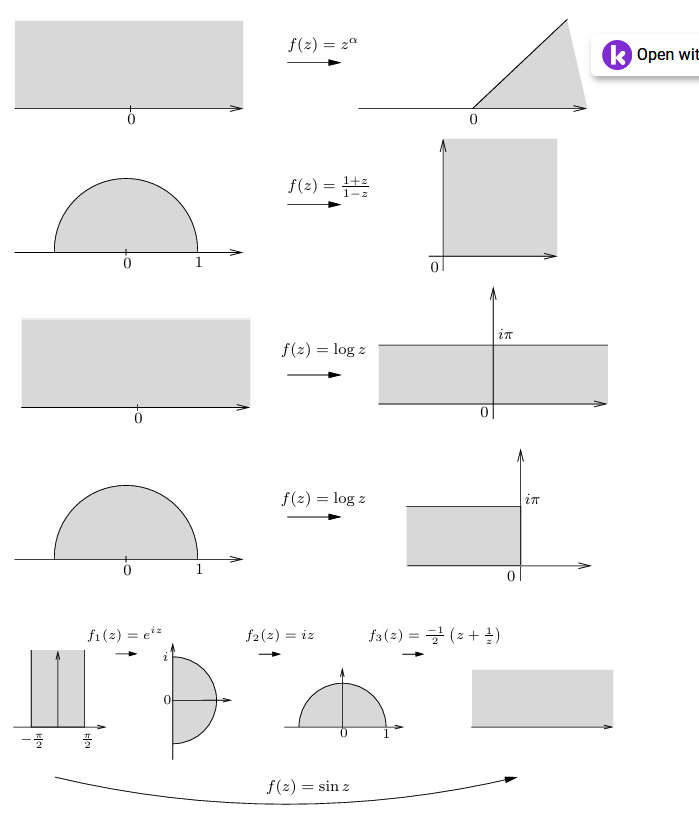
\includegraphics[width=0.5\linewidth]{Images/ComformalMaps.png}
    \caption{Conformal Maps}
\end{figure}

\begin{defn}
    A \textbf{rotation} is a map of the form $z\to cz$ where $|c| = 1$ such that $c = e^{i\varphi}$ with $\varphi \in  [0,2\pi)$
\end{defn}

\begin{lem}
    Let $f: \mathbb{D}\to \mathbb{D}$ such that $f \in H(\mathbb{D})$ and $f(0) = 0.$ Then 
    \begin{enumerate}
        \item $|f(z)| \leq |z|$ for all $z \in \mathbb{D}.$
        \item If for some $z_0 \neq 0$ we have $|f(z_0)| = |z_0|,$ then $f$ is a rotation.
        \item $|f'(0)| \leq 1.$ If $|f'(0)| = 1,$ then $f$ is a rotation.
    \end{enumerate}
\end{lem}
\begin{proof}
    About $0,$ since $f(0) = a_0 = 0,$ we use Riemann's Singularity Theorem (21) to show that 
    \[f(z) = a_1 z + a_2z^2 + \cdots \implies \frac{f(z)}{z} \in H(\mathbb{D}).\] Since $|f(z)| \leq 1,$ then 
    \[\frac{|f(z)|}{|z|}  \leq \frac{1}{|z|}\leq \frac{1}{r}\] for some $r<1.$ By the maximum modulus principle, this is true for any $|z| \leq r,$ and letting $r\to 1$ obtains the result. 

    By the first part, we have that for any $z\in \mathbb{D},$
    \[g(z) =\frac{|f(z)|}{|z|} \leq 1,\] but $g(z_0) = 1$ is the maximum and thus by the maximum modulus principle $g(z)$ is constant. Hence, 
    \[g(z)= c \implies |f(z_0)| = |c||z_0| \implies |c| = 1\]

    Define 
    \[g(z) = \frac{f(z)}{z}\] and thus 
    \[g(0) = \lim_{z\to 0}\frac{f(z) - f(0)}{z} = f'(0) \leq 1.\] Use the Maximum Modulus principle for equality.
\end{proof}

\begin{exmp}
    Let $f$ be conformal on $\{z: \Re{(z) >0}\}$ and $f(a) = a $ for some $a\in \bbR.$ Show that $|f'(a)| < 1.$

    There is some $|r|<1$ such that for $|z| < r ,$ 
    \[f(z) = f(a) + a_1(z-a) + \cdots.\] Define the map
    \[g(z) = \frac{f(z) - a}{z - a}\] which is holomorphic in $D_r(a).$ 
    By continuity, we have that $|f(z) - a| < r$ as $z \to r.$ Hence, 
    \[|g(z)| \leq \frac{1}{|r|} \to 1.\] By the maximum modulus principle, either $g(z)$ is constant or $|g(z)|< 1$ for all $z\in D_r(a).$ We are probably assuming that the map is not the constant map and so by the latter, we have that $|g(a)| < 1.$ But then 
    \[|g(a)| = \lim_{z\to a}\frac{|f(z) - a|}{|z-a|} =|f'(a)|< 1.\]

Alternatively, by the Riemann Mapping theorem, there exists some conformal map $F: \bbH_+ \to \bbD$ such that $F(a) = 0$ and $|F'(a)| >0$ Now we can consider the conformal map $\psi = F\circ f \circ F^{-1}: \bbD \to \bbD$ with $F(0) = F(f(F^{-1}(0))) = F(f(a)) = F(a)= 0.$ By the Schwarz lemma, we have that $|\psi'(0)| \leq 1.$ Expanding, we see that 
\begin{align*}
\psi'(z) &= (F(f(F^{-1}))'\\ &= F'(f(F^{-1}(z)))\cdot f'(F^{-1}(z))\cdot (F^{-1})'(z)\\
\psi'(0) &= F'(f(F^{-1}(0)))\cdot f'(F^{-1}(0))\cdot (F^{-1})'(0)\\
&= F'(f(a)) \cdot f'(a)\cdot \frac{1}{F'(F^{-1}(0))}\\
&= F'(a)\cdot f'(a) \cdot \frac{1}{F'(a)}\\
&= f'(a)
\end{align*}
and thus $|\psi'(a)| = |f'(a)| \leq 1.$ 


    \end{exmp}

\begin{defn}
We say that $f$ is an \textbf{automorphism} if it is a conformal map $f: \Omega \to \Omega$ where $\Omega$ is open. 
\end{defn}

\begin{exmp}
    Show that $f(z) = 2z + z^2$ with $z\in \mathbb{D}$ is an automorphism.

    Clearly $f \in H(\bbD).$ Suppose $f(z_1) = f(z_2).$ Then 
    \[2z_1 + z_1^2 = 2z_2 + z_2^2 \iff z_1^2 - z_2^2 + 2(z_1 - z_2) = 0\iff (z_1 - z_2)(z_1 + z_2 + 2) = 0\]
    Thus, either $z_1 - z_2 = 0$ in which case we are done, or 
    \[z_1 + z_2 + 2 = 0 \iff z_1 + z_2 = 0 \implies |z_1 + z_2| = 2\] but 
    \[|z_1 + z_2| \leq |z_1| + |z_2| < 1 + 1 = 2\] and this is a contradiction.

    Let $w\in \bbD.$ Consider $z = \sqrt{1 + w} -  1.$ Note that 
    \[2z + z^2 = w.\] TO see that $|z| < 1,$ we note that 
    \[1 + w = z^2 + 2z + 1 \iff w = z^2 + 2z = z(z + 2) \iff |w| = |z||z + 2| \leq |z|(2 + |z|) < 1\] Solving 
    \[|z|^2 + 2|z| - 1 <0,\] we see that \[|z| = -1 + \sqrt{2} < 1\]
\end{exmp}

\begin{defn}
    We say that $\Omega\subseteq \bbC$ is \textbf{proper} if it is nonempty and not $\bbC.$
\end{defn}
\begin{defn}
    Let $\mathcal{F}$ be a family of holomorphic functions. We say that $\mathcal{F}$ is \textbf{normal} if every sequence in $\mathcal{F}$ has a subsequence that converges uniformly on every compact subset of $\Omega.$
\end{defn}
\begin{defn}
    We say that $\mathcal{F}$ is \textbf{uniformly bounded on compact subsets}of $\Omega$ is for each compact $K\subset \Omega,$ there is some $B>0$ such that 
    \[|f(z)| \leq B \qquad \forall z \in K, f\in \mathcal{F}\]
 \end{defn}
 \begin{defn}
     We say that $\mathcal{F}$ is \textbf{equicontinuous} if for every $\epsilon>0,$ there is some $\delta>0$ such that  if $z,w \in K$ and $|z - w| < \delta$ then $|f(z) - f(w)| < \epsilon$ for any $f \in \mathcal{F}$
 \end{defn}
 \begin{thm}
     (Montel) Suppose $\mathcal{F}$ is a family of holomorphic functions on $\Omega$ that is uniformly bounded on compact subsets of $\Omega,$ then 
     \begin{enumerate}
         \item $\mathcal{F}$ is equicontinuous on every compact subset of $\Omega$.
         \item $\mathcal{F}$ is a normal family.
     \end{enumerate}
 \end{thm}
 \begin{proof}
     The second is simply Arzela-Ascoli. For the second, use the Cauchy Integral formula for $f(z) - f(w)$ and estimate.   
 \end{proof}

\begin{prop}
    If $\Omega$ is a connected open subset of $\bbC$ and $\{f_n\}$ is a sequence of injective holomorphic functions on $\Omega$  that converge uniformly on every compact subset of $\Omega$ to a holomorphic function $f,$ then $f$ is either injective or constant. 
\end{prop}
\begin{proof}
    Suppose not. Let $z_1, z_2 \in \Omega$ such that $z_1\neq z_2$ but $f(z_1) = f(z_1).$ Then 
    \[g_n(z) = f_n(z) - f_n(z_1) \to g(z) = f(z) - f(z_1).\] Note that 1) $g_n$ has no zeros other than $z_1$ since $f_n$ are all injective and 2) If $f$ is not constant, then $z_2$is an isolated zero for $g$ since $\Omega$ is connected. Thus, by the argument principle, for $\gamma$ small circle about $z_2,$
    \[\frac{1}{2\pi i} \int_\gamma \frac{g'}{g}d\zeta = 1\] However, we know that inside $\gamma,$
    \[\frac{1}{2\pi i}\int_\gamma \frac{g_n'}{g_n}d\zeta \to \frac{1}{2\pi i}\int_\gamma \frac{g'}{g}d\zeta = 1,\] a contradiction to the fact that $g_n$ has no zeros inside $\gamma.$ 
\end{proof}

\begin{thm}
    (Riemann Mapping Thm) Suppose $\Omega$ is proper and simply connected. If $z_0 \in \Omega,$ then there exists a unique conformal mapping $F: \Omega \to \mathbb{D}$ such that 
    \[F(z_0) = 0 \qquad F'(z_0) >0\]
\end{thm}
\begin{proof}
    We show uniqueness first. Let $F,G: \Omega \to \mathbb{D}$ be conformal. Then consider $H = F \circ G^{-1}$ to be the automorphism of the disk fixing the origin. By the Schwarz Lemma, we have that $H(z) = e^{i\varphi} z$ is a rotation, but since $H'(0) >0,$ then $e^{i\varphi} = 1,$ and thus $F = G$

    \textit{Step 1} In this step, we will show $\Omega$ is conformally equivalent to some $U \subseteq \mathbb{D}$ open such that $0 \in U.$ Since $\Omega \neq \bbC,$ let $\alpha \in \bbC \sm \Omega.$ Since $z-\alpha \neq 0$ for any $z\in \Omega,$ we define $f(z)= \log(z - \alpha)$ to be holomorphic on $\Omega.$ It is not hard to see $f$ is injective. Let $w \in \Omega.$ Assume that $f(z) = f(w) + 2\pi i,$ then exponentiating, 
    \[z-\alpha=e^{f(z)} = e^{f(w)} = w-\alpha,\] an obvious contradiction. We actually claim something much stronger, that there is some disk about $f(w)+ 2\pi i$ containing no points of $f(\Omega).$ Suppose not, then there is a sequence $f_n(z)\to f(w) + 2\pi i,$ exponentiating yields a sequence $z_n \to w$ and by continuity of $f$ implies $f(z_n)\to f(w),$ which we have seen is a contradiction. Hence, there is a disk about $f(w) + 2\pi i$ such that $f(z) - (f(w) - 2\pi i)$ doesn't vanish, and so we can define $F: \Omega \to \bbC$ by 
    \[F(z) = \frac{1}{f(z) - (f(w) - 2\pi i)}\] which is injective since $f $ is injective. Thus, $F: \Omega \to F(\Omega)$ is conformal. By dilating it and traslating it, we obtain $F: \Omega \to U.$

    \textit{Step 2} By step 1, we assume WLOG that $\Omega \subseteq \mathbb{D}$ is open and contains the origin. Let 
    \[\mathcal{F}:= \{f: \Omega \to \mathbb{D} \mid f \text{ injective, holomorphic, $f(0) = 0$}\}\]
Because of the identity map, $\mathcal{F}\neq \emptyset,$ and because $\|f\| \leq 1$ for any $f \in \cal F,$ then $\cal F$ is uniformly bounded. Moreover, we apply the Cauchy Integral formula to uniformly bound $|f'(0)|.$ Hence $s = \sup_{f\in \cal F} |f'(0)|$ exists. Choose a sequence $f_n \subset \cal F$ such that $|f_n'(0)|\to 0.$ By Montel's Theorem (Arzela-Ascoli), there exists a subsequence that converges uniformly on compact sets of $\Omega$ to some function $f.$ We know that $s \geq 1$ since $z\mapsto z$ is in $\cal F,$ and thus $f$ cannot be constant, and thus by the previous proposition, $f$ must be injective. We know by continuity that $|f(z)| \leq 1,$ but the Maximum Modulus principle tells us that the inequality is actually strict. Since $f(0) = 0,$ we know that $f \in \cal F$ with $|f'(0)| = s.$   

\textit{Step 3} It remains to see that the $f$ from step 2 is conformal into $\mathcal{D}.$ We know that $f$ is holomorphic by Morera's theorem, and we know it to be injective by step 2, so it suffices to show surjective. This is weird and  doesn't contribute to anything so I'm good.
    
\end{proof}

\begin{cor}
    Any two proper and simply connected sets are conformally equivalent. If $z \in U$ and $w \in V,$ then $f(z) = w$ and $f'(z) >0.$ 
\end{cor}
\begin{proof}
    Let $U,V$ be proper and simply connected. By the Riemann Mapping Thm, there exist $F,G$ conformal maps such that $F: U \to \mathbb{D}$ and $G: V\to \mathbb{D}.$ Define $H: U\to V$ by $H = G^{-1}\circ F.$ We know that $G^{-1}$ is conformal by remark 21, and clearly a composition of conformal maps is conformal. 
\end{proof}

\begin{exmp}
    Let $\Omega \subseteq \bbC$ be a simply connected domain. Let $z_1, z_2 \in \Omega.$ Show there exists an automorphism such that $f(z_1) = z_2.$ 

    We simply apply the Riemann mapping theorem if $\Omega \neq \bbC$ and use the Mobius automorphism of the disk
    \[\varphi_\alpha(z) = \frac{z-\alpha}{1-\bar\alpha z}\]
    Suppose now $\Omega = \bbC.$ Then consider $f(z) = z - z_1 + z_2.$ Then $f$ is clearly an automorphism with $f(z_1) = z_2.$
\end{exmp}

\begin{exmp}
    Let $H_t = \mathbb{H}\sm [0, 2\sqrt{t}i].$ Let $g_t : H_t \to \mathbb{H}$ be defined such that 
    \[g_t(z) = \sqrt{z^2 + 4t},\] then $g_t$ is a conformal. As $z\to \infty,$ 
    \[|sqrt{z^2 - 4t}\to z,\] and thus $g_t$ looks like the identity map for large $z.$ Consider the ODE 
    \begin{align}
\partial_t f_t (z) = \frac{2}{f_t(z)}, \qquad f_0(z)= z        
    \end{align}
 We claim that $g_t$ is a solution. Clearly the boundary condition is satisfied. Taking the partial, 
    \[\partial_t g_t(z) = \frac{1}{2\sqrt{z^2 + 4t}}\cdot 4 = \frac{2}{g_t(z)}.\] Before the denominator in $(3)$ implodes, theorems in ODE (Picard-Lindelof) imply that $g_t$ is the unique solution to (3). Hence, the geometry of the curve $\gamma(t) = 2\sqrt{t}i$ is completely encoded by $g_t.$
\end{exmp}

\newpage
\subsection{Distortion Estimates}

\begin{rem}
    Recall that $f = u + iv$ is holomorphic iff it satisfies the Cauchy-Riemann equations:
    \[\frac{\partial u}{\partial x} = \frac{\partial v}{\partial y} \qquad \frac{\partial u}{\partial y} = - \frac{\partial v}{\partial x}.\] In particular, we have showed that this implies that 
    \[\triangle u = \frac{\partial^2}{\partial x^2}u + \frac{\partial^2}{\partial y^2} u  = 0 \qquad \triangle v = 0\]
\end{rem}
\begin{defn}
    We say that $f$ is \textbf{harmonic} if $\triangle f = 0.$
\end{defn}

\begin{defn}
    We say that a process $B = B^1 + iB^2$ is a \textbf{complex Brownian motion} if $B^1, B^2$ are independent S.B.M in $\bbR.$ 
\end{defn}
Recall the following theorem from probability:
\begin{thm}
    Let $u$ be a harmonic function on a bounded domain $D$ continuous on $\overline{D}.$ Then $u(B_t)$ is a martingale. 
\end{thm}
\begin{rem}
    We can use the continuous time OST to see that if $\tau = \inf\{t \geq 0 \mid B_t  \notin D\}$ is the first time $B_t$ leaves $D,$ then 
    \[\bbE[u(B_\tau)] = \bbE[u(B_0)] = u(z)\]
\end{rem}
We recall a few theorems we have already shown. In the context of the previous theorem, $u$ is harmonic and thus is holomorphic and thus, 
\begin{enumerate}
    \item (Mean value property) \[u(z_0) = \frac{1}{2\pi i}\int_0^{2\pi} u(z_0 + re^{i\theta})d\theta.\]
    \item (Maximum Modulus) If the $u$ attains its maximum on the interior of $D,$ then $u$ is constant. 
\end{enumerate}
For notation, if we let $D \subseteq \bbC$ be any proper and simply connected set containing the origin, we define 
\[\mathcal{U}:= \{f: \mathbb{D}\to D\mid f \text{conformal s.t. } f(0) = 0, f'(0) = 1\}\]
If $f\in U,$ then $f$ is analytic with $a_0 = 0, a_1 = 1$ and thus 
\[f(z) = z+ \sum_{n=2}^\infty a_n z^n\]
\begin{lemma}
    If $f\in \cal U,$ there exists an odd function $h \in \cal U$ such that $h(z)^2 = f(z^2).$
\end{lemma}
\begin{proof}
    Recall that $h$ is odd if $h(-z) = -h(z).$ Define 
    \[\tilde{f}(z) = \begin{cases}
        \frac{f(z)}{z}\qquad z\neq 0\\
        f'(0)\qquad z = 0
    \end{cases}\] Since $\tilde{f}$ is conformal and never vanishes, we can express
    \[\tilde{f}(z)= e^{\log \tilde{f}(z)}\] and so we can define 
    \[g(z) := e^{\frac{1}{2}\log \tilde{ f}(z)} \implies g(z)^2= \tilde{f}(z).\] Define now 
    \[h(z):= zg(z^2).\] Notice that $h$ is odd since 
    \[h(-z) =-zg((-z)^2)= -zg(z^2) = -h(z)\] and that 
    \[h(z)^2 = z^2 g(z^2) = z^2 \tilde{f}(z^2) = f(z^2).\] It remains to show that $h\in \cal U.$ This is not hard to show.
\end{proof}

\begin{prop}
    If $f \in \cal U,$ then 
    \[\text{area} (f(\mathbb{D})) = \pi  \sum_{n=1}^\infty n |a_n|^2\]
\end{prop}
\begin{proof}
    Let $C$ be the circle of radius $r$ and let $\gamma  = f(C).$ Then 
    \begin{align*}
        \frac{1}{2i} \int_\gamma \overline{z} \,dz &= \frac{1}{2i}\int_\gamma (x - iy)(dx + i\,dy)\\
        &= \frac{1}{2i}\int_\gamma (x - iy)\,dx + (ix + y)\,dy\\
        &= \frac{1}{2i}\int \int_{f(r\mathbb{D})}2i\,dxdy\\
        &= \text{area}(f(r\mathbb{D}))
    \end{align*}
    by the Green's Theorem. But by definition, we have that 
\begin{align*}
    \frac{1}{2i}\int_\gamma \overline{z}\,dz &= \frac{1}{2i}\int_0^{2\pi}\overline{f(re^{i\theta})}f'(re^{i\theta})ire^{i\theta}\,d\theta\\
    &= \frac{1}{2i} \int_0^{2\pi} \sum_{n=1}^\infty \overline{a_n} r^n e^{{-i\theta n}} \sum_{n=1}^\infty n{a_n} r^{n-1} e^{{i\theta (n-1)}} ir^{i\theta}d\theta\\
    &= \pi \sum_{n=1}^\infty r^{2n}|a_n|^2 n
\end{align*}
Letting $r\to 1$ proves the result.
\end{proof}

\begin{defn}
    Let $K\subseteq \bbC$ be compact and connected. Then $K$ is a \textbf{compact hull} if $\bbC \sm K$ is connected and $K$ consists of more than a single point. 
\end{defn}
\begin{rem}
    Note  by the Riemann Mapping Thm, there exists some $F: \bbC \sm \overline{D} \to \bbC \sm K$ such that $F$ is bijective and conformal and such that fixes $\infty$ and $\lim_{z\to \infty} \frac{F(z)}{z} >0.$ To see this we call $I(z) = \frac{1}{z},$ and $f: \bbD \to I(\bbC \sm K)$ to be the conformal map with $f'(0)>0,$ then 
    \[\frac{F(z)}{z} = \frac{1}{zf(\frac{1}{z})} \xrightarrow[]{z\to \infty} \frac{1}{f'(0)} >0\]
    Define 
    \[\mathcal{H}:= \{K \text{ compact hull }\mid \lim_{z\to \infty}  \frac{F(z)}{z} = 1\}\] Thus, if $K \in \cal H,$ then the Laurent expansion of $F$ is 
    \[F(z) = \sum_{n=0}^\infty \frac{b_n}{z^n} + \sum_{n=1}^\infty a_nz^n \] but imposing our condition implies that $a_n = 0$ for all $n>1$ and that $a_1 = 1.$ Thus, 
    \[F(z) = z + a_0 + \sum_{n=1}^\infty \frac{b_n}{z^n}\]
\end{rem}

\begin{prop}
    Suppose $K \in \cal H,$ then 
    \[\text{area}(K) = \pi(1 - \sum_{n=1}^\infty n |b_n|^2).\] Since area is non-negative, we must have that $\sum_{n=1}^\infty n |b_n|^2 \leq 1.$ 
\end{prop}
\begin{proof}
    Letting $r>1$ and $K_r = F(r\overline{\bbD})$ (rather, $K_r$ is the image of the annulus $r\overline{\bbD}\sm \bbD$). Since $F$ is bijective, then as $r\to 1,$ $F(r\overline{\bbD})\to \bbC\sm K.$ Hence, it suffices to find that $\text{area}(K_r).$ Letting $\gamma = F(re^{i\theta}),$ we compute 
    \begin{align*}
        \text{Area}(K_r) = \frac{1}{2i}\int_\gamma \overline{z} \,dz\\
        &= \frac{1}{2i}\int_{0}^{2\pi} \overline{F(re^{i\theta})}F'(re^{i\theta})ire^{i\theta}\,d\theta\\
        &= \pi(r^2 - \sum_{n=1}^\infty n |b_n|^2 r^{-2n})\\
        &\to \pi(1 - \sum_{n=1}^\infty n|b_n|^2)
    \end{align*}
\end{proof}



\begin{prop}
    If $f \in \cal U,$ then $|a_2| \leq 2.$ 
\end{prop}
\begin{proof}
    Define $h$ as in the previous lemma. Since it is odd, its expansion about $0$ has no even powers of $z.$ Thus, we can express
    \[h(z) = z + c_3 c^3 + c_5z^5 + \cdots\] Since $f(z^2) = h(z)^2,$ we have that 
    \[z^2 + a_2z^4 + \cdots = (z + c_3 c^3 + c_5z^5 + \cdots) = z^2 + 2c_3z^4 + \cdots\] implying that $c_3 = \frac{a_2}{2}.$ Defining $g(z) = \frac{1}{h(\frac{1}{z})},$ we see that 
    \[g(z) = \frac{1}{z^{-1} + (\frac{a_2}{2})z^{-3} + \cdots} = z - \frac{a_2}{2}z^{-1} + \cdots \]
    By Proposition 14, 
    \[|\frac{a_2}{2}|^2 \leq 1 \implies |a_2| \leq 2\]
\end{proof}

\begin{thm} (Koebe$-\frac{1}{4}$)
    If $f\in \cal U,$ $0<r\leq 1,$ then $B_{\frac{r}{4}}(0)\subseteq f(r\mathbb{D})$
\end{thm}
\begin{proof}
    Let $r = 1$ and let $z_0 \notin D.$ It suffices to show for this case that $|z_0| \geq \frac{1}{4}.$ Define 
    \[\tilde{f}(z) = \frac{z_0 f(z)}{z_0 - f(z)}.\] To see that $\tilde{f} \in \cal U,$ notice that $\tilde{f}(0) = 0$ and 
    \[\tilde{f}'(z) = \frac{z_0f'(z)(z_0 - f(z)) + z_0f(z)'f(z)}{(z_0 - f(z))^2} \implies \tilde{f}'(0) = \frac{z_0^2 f'(0)}{z_0^2} = 1.\] Writing $f(z) = z + \sum_{n=2}^\infty a_n z^n,$ 
    \[\tilde{f}(z) = \frac{z_0(z + a_2z^2 + \cdots)}{z_0 - (z - a_2z^2 + \cdots)}= (z + a_2z^2)\frac{1}{1 - \frac{z}{z_0} + \frac{z^2}{z_0^2} + \cdots} \] recognizing the last term as geometric, 
    \[\tilde{f}(z) = (z + a_2z^2)(1 + \frac{z}{z_0} + \cdots) = z + \frac{z^2}{z_0} + a_2z^2 + \cdots = z + (a_2 + \frac{1}{z_0})z^2 + \cdots\] From the last proposition, we have that 
    \[|a_2| \leq 2 \quad |a_2 + \frac{1}{z_0}| \leq 2 \implies |z_0| \leq \frac{1}{4}\] as desired. Now let $r \in (0,1).$ Consider the conformal map $g(z) = \frac{f(rz)}{r}.$ Let $|z| < \frac{1}{4} \implies z \in g(\bbD) = \frac{f(r\mathbb{D})}{r}$ and thus we are done.
\end{proof}

\begin{cor}
    Suppose $D, \tilde{D}\subset \bbC$ and $z \in D$ and $\tilde{z}\in \tilde{D}$ and $f D \to \tilde{D}$is conformal with $f(z) = \tilde{z}.$ Then if $d = \text{dist}(z, \partial D)$ and $\tilde{d}= \text{dist}(\tilde{z}, \partial \tilde{D}),$ we have that 
    \[\frac{\tilde{d}}{4d} \leq |f'(z)| \leq \frac{4\tilde{d}}{d}.\]
\end{cor}
\begin{proof}
    We assume WLOG that $z = \tilde{z} = 0.$ Letting 
    \[[\tilde{f}(w) = \frac{f(dw)}{df'(0)},\] we note that $\tilde{f} \in \cal U$ and thus by Koebe's theorem, 
    \[B_{\frac{r}{4}}(0) \subseteq \tilde{f}(r\mathbb{D}).\] Thus, for every $\epsilon>0,$ there is some $\delta>0$ such that $w \in \mathbb{D}\sm (1-\delta)\mathbb{D} = \mathbb{D}\sm r\mathbb{D},$ we have that 
    \[|\frac{f(dw)}{df'(0)}| = |\tilde{f}(w)| \geq \frac{1}{4} - \epsilon = \frac{r}{4}\] Taking the infemum over all such $w,$ we see that 
    \[\frac{\tilde{d}}{d|f'(0)|} \geq \inf _{w \in \mathbb{D}\sm (1-\delta)\mathbb{D}}|f'(w)|  \geq \frac{1}{4} - \epsilon.\] Taking $\epsilon\to 0$ and rearranging 
    \[\frac{4\tilde{d}}{d} \geq |f'(0)|.\] The lower bound follows from the same logic with $f^{-1}.$
\end{proof}

\newpage
\subsection{Half-Plane Capacities}
\begin{thm}
    (Shwarz Reflection Principle) Let $\Omega =\{z \in \Omega \mid \Im{z} >0\}$. Suppose $f: \Omega^+ \to \bbC$ is continuous to $\bbR$ such that $f$ is real valued on $\bbR,$ then there is a function $F \in H(\Omega)$ such that $F = f$ on $\Omega.$ 
\end{thm}
\begin{proof}
    Define $F(z)$ for $z\in \Omega^-$ by 
    \[F(z) = \overline{f(\overline{z})}\] Then since $f$ is analytic, we have that if $z_0, z_1 \in \Omega^{-},$ then their conjugates are clearly in $\Omega^+$ and so
    \[F(z) = \overline{\sum_{n=1}^\infty a_n (\overline{z}_0 - \overline{z}_1)^n} = \sum_{n=1}^\infty \overline{a}_n (z_0 - z_1)^n.\] Thus, $F\in H(\Omega^{-1})$ and it extends continuously to $\bbR$ since $\overline{f(x)} = f(x)$ since $f$ is real valued on $\bbR.$ Let $T$ be a triangle. If $T$ lies entirely on $\Omega^{-}$ or $\Omega^+,$ then $\int_T F(z)\,dz = 0$ by Cauchy's theorem. Suppose an edge of $T$ lies on $\bbR.$ Then call $T_\epsilon$ to be the triangle a tiny bit up and thus by continuity,
    \[0 = \int_{T_\epsilon} F(z)\,dz \to \int_{T} F(z)\,dz.\] By Morera's Theorem, we are done. 
    \begin{figure}[H]
        \centering
        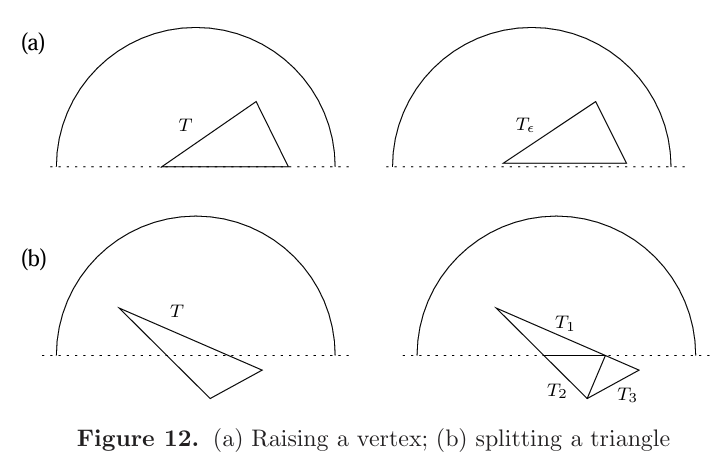
\includegraphics[width=0.5\linewidth]{Images/Symmetry Principle.png}
        \caption{Proof idea}
    \end{figure}
\end{proof}
\begin{cor}
    Let $D\subseteq \bbH$ be a simply connected domain and $\phi: D\to \bbH$ be a conformal transformation bounded on bounded sets. Then $\phi $ extends by reflection to a conformal transformation on $D^* = D\cup \{\overline{z}:z \in D\}\cup(\overline{D} \cap \{ \in \partial H\})$
\end{cor}

\begin{defn}
    A set $A \subseteq \bbH$ is called a \textbf{compact $\bbH-$hall} if $A = \bbH \cap \overline{A}$ and $\bbH \sm A$ is simply connected. We denote 
    \[\mathcal{Q} = \{A \subseteq \bbH \mid A \text{ compact hull}\}\]
\end{defn}
\begin{prop}
    For each $A\in \cal Q,$ there exists a unique conformal transformation $g_A:\bbH \sm A \to \bbH$ such that $|g_A(z) - z|\to 0$ as $z\to \infty.$
\end{prop}
\begin{proof}
    The Riemann Mapping Thm takes care of the first part, giving us some $g: \bbH\sm A \to \bbH $ and the fact that $|g(z)|\to \infty $ as $|z|\to \infty$ (this might mean that we compose $g$ with something as well but it's fine). By setting $g(\overline{z}) =\overline{g(z)}$, the Schwarz Reflection Principle tells us we can shave off more of the domain, extending $g$ to be defined on $\bbC \sm (\{\overline{z} : z\in A\}\cup \overline{A}).$ The Laurent expansion of $g$ becomes (as we showed in Remark 24)
    \[g(z) = a_0 + a_1z + \sum_{n=1}^\infty \frac{b_n}{z^n}.\] If $z\in \bbR,$ then $\bar z = z$ and by how we defined $g,$ $g(z) = g(\bar z) = \overline{g(z)}.$ Let $z\in \bbR \sm \overline{A},$ then since $g(z) \in \bbR,$ we can expand $g(z)$ to be
    \[a_0 + a_1 z + \sum_{n=1}^\infty \frac{b_n}{z^n} = \overline{a_0} + \overline{a_1} z + \sum_{n=1}^\infty \frac{\overline{b_n}}{z^n} \] implying that each coefficient is real. Now define 
    \[g_A(z) := \frac{g(z) - a_0}{a_1} = z + \sum_{n=1}^\infty \frac{c_n}{z^n}.\] Hence, $|g_A(z) - z|\to \infty$

    Since the group of automorphisms of $\bbH$ is of the form 
    \[\frac{az + b}{cz + d}\] where $a,b,c,d \in \bbR$ and $ad - bc = 1$ then if $g_A, \tilde{g}_A: \bbH \sm A \to \bbH$ are two maps with the property that they look identical to $z$ at infinity, then $g_A \circ \tilde{g}^{-1}_A: \bbH \to \bbH$ is of the form 
    \[g_A \circ \tilde{g}^{-1}_A = \frac{az+b}{cz + d}\] and 
    \[\left| \frac{az+b}{cz + d} - z\right| \to 0 \implies a = c = 1, b = d = 0\] Hence, $g_A$ is an inverse of $\tilde{g}^{-1}$ and so we are done.
\end{proof}

\begin{defn}
    Let $A\in \cal Q.$ We define the \textbf{half-plane} capacity of $A$ to be 
    \[\hcap(A) = \lim_{z\to \infty} z(g_A(z) -z).\]
\end{defn}
\begin{rem}
    Equivalently, we can see that by rearranging, 
    \[g_A(z) =z + \frac{\hcap(A)}{z} \]
    
    
    since 
    \[z(g_A(z)-z) =z(z + \sum_{n=1}^\infty \frac{c_n}{z^n} -z_ ) = c_1 + \frac{c_2}{z} + \cdots \to c_1\] Thus, 
    \[\hcap(A) = c_1.\]
\end{rem}
\begin{exmp}
    Consider $A = [0, 2\sqrt{t}i].$ Recall that $g_A: \bbH \sm A \to \bbH$ is 
    \[g_A(z) = \sqrt{z^2 + 4t}\] with $|\sqrt{z^2 + 4t} - z|.$ Expanding, we see that 
    \[g_A(z) = z\sqrt{(1 + \frac{4t}{z^2})} = z(1 + \frac{2t}{z^2} + \cdots)\] and thus 
    \[\hcap(A) = 2t\]
\end{exmp}

\begin{exmp}
    (Upper disk). Consider that $g_{\overline{\bbD}\cap \bbH}(z) = z + \frac{1}{z}$ is the conformal transformation $\bbH\sm \overline{\bbD}\to \bbH$ with $\hcap (\overline{\bbD}\cap \bbH) = 1$
\end{exmp}
\begin{prop}
    The following hold:
    \begin{enumerate}
        \item Let $r>0,$ then $\hcap(rA) = r^2\hcap(A)$
        \item Let $x\in \bbR$. Then $\hcap(A + x) = \hcap (A)$
        \item Suppose $A\subseteq \hat A,$ then $\hcap(A) \leq \hcap (\hat A)$
    \end{enumerate}
\end{prop}
\begin{proof}
    (i) Let 
    \[g_A = z + \frac{c_1}{z} + \cdots \] such that $\hcap (A)= c_1.$ It suffices to show that $\hcap (rA) = r^2 c_1.$ To see this, we note that, 
    \[g_{rA}(z) = rg_A(\frac{z}{r}) = r(\frac{z}{r} + \frac{c_1}{\frac{z}{r}} + \cdots ) = z + \frac{r^2 c_1}{z} + \cdots\] and we are done.

    (ii) This is obvious by considering that $g_A(z - x) + x: \bbH \sm (A + x)\to \bbH$ is the conformal transformation. 

    (iii) Ask Yearwood
\end{proof}
\begin{rem}
    If $A\subseteq r\overline{\bbD} \cap \bbH,$ then $\hcap (A) \leq \hcap (r\overline{\bbD}\cap \bbH) = r^2 \hcap(\overline{\bbD}\cap \bbH) = r^2$
\end{rem}

\begin{thm}
    Suppose $A \in \cal Q,$ $B$ is a complex Brownian motion, $\tau$ is the first exit time of $B$ from $\bbH \sm A.$ Then 
    \begin{enumerate}
        \item For all $z\in \bbH \sm A, $ $\Im{(z - g_A(z))} = \bbE[\Im{(B_\tau) \mid B_0 = z}]$
        \item $\hcap(A) = \lim_{y\to \infty} y \bbE[\Im{(B_\tau)} \mid B_0 = iy]$
        \item 
        \[\hcap(A)  = \frac{2}{\pi} \int_0^\pi \bbE[\Im{(B_\tau)\mid B_0 = e^{i\theta}}] \sin \theta \,d\theta\]
    \end{enumerate}
\end{thm}
\begin{proof}
    (a) Note that for any $w\in \partial (\bbH \sm {A}),$ we have that $\Im(g_A(z)) = 0.$ 
    
    We have showed that $\Im(\cdot)$ is harmonic by the Cauchy-Riemann equations. Thus, we can apply Remark 23 to see that since $z - g_A(z)$ is holomorphic, then $\Im(z - g_A(z))$ is harmonic and thus 
    \[\Im(z -g_A(z)) = \bbE[\Im{B_\tau - g(B_\tau)} \mid B_0 = z]\] 

    
    (b) Recall that $\Re(iz) = \Im(ix -y)  = -\Im(z).$ Applying this to the fact that $\hcap(A)$ is real then by taking the real part of the following expression
    \[\hcap(A) = \lim_{z\to \infty} z(g_A(z) - z) = \lim_{y\to \infty} iy(g_A(iz) - iy)\] we see that 
    \[\hcap(A) = \lim_{y\to \infty} y\Im(iy - g_A(iy)) = \lim_{y\to \infty}y \bbE[\Im(B_\tau)\mid B_0 = iy]\] where the last equality comes from part 1.

    (c) 
\end{proof}

If $f$ is conformal, then $f(B)$ is a Brownian motion. Basically:
\begin{thm}
    Let $D, \tilde{D}\subseteq \bbC$ and $f: D\to \tilde{D}$ be conformal. Let $B, \tilde{B}$ be complex Brownian motions starting from $z\in D$ and $\tilde{z}= f(z) \in \tilde{D}.$ Denoting the exit times by 
    \[\tau = \inf\{t\geq 0 \mid B_t \notin D\} \qquad \tilde{\tau} = \inf\{\tilde{B}_t \notin \tilde{D}\}\]  we set 
    \[\tau' = \int_0^\tau |f'(B_s)|^2 \,ds \qquad \sigma(t) = \inf\{s\geq 0 : \int_0^s |f'(B_r)|^2 = t\}\] for $t< \tau'$. Setting $B_t' = f(B_{\sigma(t)})$, 
    \[(\tau', B_t' : t< \tau ') =^d= (\tilde{\tau}, \tilde{B}_t: t< \tilde{\tau})\]
\end{thm}
\begin{rem}
    Here are a few facts I might prove:
    \begin{itemize}
        \item The first exit time distribution of $B$ starting at $0 \in \bbD$ in $\bbD$ is given by a uniform distribution on $\partial D.$
        \item If now we start at $z\in \bbD,$ the distribution is given by 
        \[\frac{1}{2\pi} \frac{1 - |z|^2}{|e^{i\theta}- z|^2}\qquad \theta \in [0,2\pi).\]
        \begin{proof}
            Let 
            \[\varphi_z(w) = e^{i\theta}\frac{z-w}{1-\bar z w}\] be the automorphism such that $z\mapsto 0.$ Consider that by the above theorem, $V = \varphi_z(B_\tau) \sim \text{Uniform}(2\pi).$ And consider $U = B_\tau = \varphi^{-1}(V).$ We seek 
            \[f_U(u) = f_V(\varphi(u))\left|\varphi_z'(u)\right| = \frac{1}{2\pi} \frac{-1 - |z|^2}{|1 - \bar z u|^2} = \frac{1}{2\pi} \frac{-1 - |z|^2}{|u-z|^2} = \frac{1}{2\pi}\frac{-1 - |z|^2}{|e^{i\theta} - z|^2}\]
        \end{proof}
        \item Starting from $z = x + iy \in \bbH,$ 
        \[\frac{1}{\pi} \frac{y}{(x- u)^2 + y^2} \qquad u \in \partial \bbH\]
    \end{itemize}
\end{rem}

\begin{defn}
    Let $A\in \cal Q.$ We define the radius of $A$ to be 
    \[\rad(A) =\sup\{|z| : z \in A\}\]
\end{defn}

\begin{prop}
    Suppose that $A\in \cal Q,$ $B$ is a complex Brownian motion, and $\tau = \inf \{t \geq 0 : B_t \notin \bbH \sm A\}.$ Then 
    \[g_A(x) = \lim_{y\to \infty} \pi y\left(\frac{1}{2} - \bbP\{B_\tau \in [x, \infty) \mid B_0 = iy\}\right) \qquad x>\rad (A)\]
    \[g_A(x) = \lim_{y\to \infty} \pi y\left(-\frac{1}{2}+ \bbP\{B_\tau \in (-\infty, x] \mid B_0 = iy\}\right) \qquad x<-\rad (A)\]
\end{prop}

\begin{proof}
    Suppose $A = \emptyset.$ We have that $g_\emptyset: \bbH \to \bbH$ with $g_\emptyset(z) = z$ satisfies $|z - z|\to 0$ as $z\to \infty.$ Using symmetry and a weird little result, if we suppose $x> 0,$
    \begin{align*}
        \pi y \left(\frac{1}{2} - \bbP\{B_\tau \in [x, \infty) \mid B_0 = iy\}\right) &= \pi y \pi y\bbP\{B_\tau \in [0,x]\}\\
        &= \lim_{y\to \infty}\int_0^x \frac{y}{\pi (s^2 + y^2)}\,ds\\
        &\xrightarrow[y\to \infty]{}x\\
        &= g_A(x)
    \end{align*}

    Suppose now $A \neq \emptyset.$ Let $g_A = u_A + iv_A$ and $\sigma = \inf \{t \geq 0 : B_t \notin \bbH\}.$ We know that 
    \[\bbP_{iy}\{B_\tau \in [x, \infty)\} = \bbP_{g_A(iy)}\{B_\sigma \in [g_A(x), \infty)\} = \bbP_{iv_A(iy)}\{B_\sigma  \in [g_A(x)- u_A(iy), \infty)\}\]
\end{proof}

\begin{cor}
    Suppose that $A\in \cal Q$ with $\rad(A) \leq 1,$ then 
    \[x \leq g_A(x) \leq x + \frac{1}{x} \qquad x>1\]
    \[x + \frac{1}{x} \leq g_A(x) \leq x \qquad x<-1\] If $A \in \cal W,$ then $|g_A(z) - z| \leq 3\rad(A)$ for all $z\in \bbH \sm A.$ 
\end{cor}
\begin{prop}
    There is some $c>0$ so that for any $A\in \cal Q$ and $|z| \geq 2 \rad(A),$ 
    \[\left|g_A(z) - z - \frac{\hcap(A)}{z}\right| \leq c \frac{\rad(A)\hcap (A)}{|z|^2}\]
\end{prop}
\begin{proof}
    Suppose $\rad(A) = 1.$ Let $h(z) = g_A(z) - z - \frac{\hcap(A)}{z}.$ Recall that 
    \[\Im(\frac{1}{z}) = \Im(\frac{1}{x+ iy}) = -\frac{y}{x^2 + y^2}\]
    
    Let 
    \[v(z) = \Im(h(z)) = \Im(z - g_A(z)) - \Im(z)\hcap(A) = \Im(z - g_A(z)) - \frac{y\hcap(A)}{x^2 + y^2}.\] Letting $B_t$ be a complex Brownian motion and $\sigma$ and $\tau$ being exit times from $\bbH \sm A.$ Let $\theta \in [0,2\pi],$ and let $p(z, e^{i\theta})$ be the density at $e^{i\theta}$ for $B_\sigma.$ By Theorem 37, we have that 
    \[\Im(z - g_A(z)) = \bbE_z[\Im(B_\sigma)] = \bbE[\bbE[\Im(B_\tau )\mid \tau = e^{i\theta}]] = \int_0^\pi \bbE_{e^{i\theta}}[\Im(B_\tau)]p(z, e^{i\theta})d\theta\]


    From an example problem, we know that 
    \[p(z, e^{i\theta}) = \frac{2}{\pi}\frac{\Im(z )}{|z|^2}\sin\theta (1 + O(|z|^{-1}))\]
    \[\hcap(A)  = \frac{2}{\pi} \int_0^\pi \bbE[\Im{(B_\tau)\mid B_0 = e^{i\theta}}] \sin \theta \,d\theta\] Plugging in, 
    \begin{align*}
        |v(z)| &= \left|\Im(z - g_A(z)) - \frac{y\hcap(A)}{x^2 + y^2}\right|\\
        &= \left|\int_0^\pi \bbE_{e^{i\theta}}[\Im(B_\tau)]p(z, e^{i\theta})d\theta - \frac{2}{\pi}\frac{\Im(z)}{|z|^2}\int_0^\pi \bbE[\Im{(B_\tau)\mid B_0 = e^{i\theta}}] \sin \theta \,d\theta\right|\\
        &=\left|\int_0^\pi \bbE_{e^{i\theta}}[\Im(B_\tau)]\frac{2}{\pi}\frac{\Im(z )}{|z|^2}\sin\theta (1 + O(|z|^{-1}))d\theta - \frac{2}{\pi}\frac{\Im(z)}{|z|^2}\int_0^\pi \bbE[\Im{(B_\tau)\mid B_0 = e^{i\theta}}] \sin \theta \,d\theta\right|\\
        &=\frac{\hcap(A)\Im(z)}{|z|^3}c
    \end{align*}
\end{proof}

\begin{thm}
    There exists a constant $c>0$ such that the following holds. Let $A\subseteq \bar \bbD$ be connected with $0 \in A$ and $A\cap \partial \bbD \neq \emptyset.$ Then 
    \[\bbP_z(B([0, \tau]) \cap A = \emptyset) \leq c\sqrt{|z|}\]
\end{thm}
\begin{prop}
    Suppose $A,\tilde{A} \in \cal Q$ where $A\subseteq \tilde{A}$ and $\tilde{A}\sm A$ is connected. Then there is some $c>0$ such that
    \[\text{diam}(g_A(\tilde{A}\sm A)) \leq c \begin{cases}
        d^\frac{1}{2}r^\frac{1}{2} \qquad d\leq r\\
        \text{rad}(\tilde{A}) \,\quad d>r
    \end{cases},\]
    where $d = \text{diam}(\tilde{A}\sm A)$ and $r = \sup\{\Im(z) : z\in \tilde{A}\}$
\end{prop}
\begin{proof}
    We assume WLOG that $r = 1.$ Consider the case when $d>1.$ We know from a previous corollary that 
    $|g_A(z) - z|< 4\rad(A).$ Hence, 
    \[\text{diam}(g_A(\tilde{A}\sm A))  \leq \text{diam}(\tilde{A}) + 6\rad(A) \leq 8\rad(\tilde{A})\]
\end{proof}

\newpage
\subsection{The Chordal Lowener Equation}
\begin{defn}
    Suppose that $(A_t) = (A_t)_{t\geq 0}$ is a family of compact $\bbH-$hulls. We say that $(A_t)$ is 
    \begin{enumerate}
        \item \textbf{non-decreasing} if $0\leq s \leq t < \infty$ implies $A_s \subseteq A_t$
        \item \textbf{locally growing} if gor every $T, \epsilon>0,$ there is some $\delta>0$ such that $0 \leq s \leq t \leq s + \delta \leq T$ so that $\text{diam}(g_{A_s}(A_t \sm A_s)) \leq \epsilon.$
\begin{figure}[H]
        \centering
        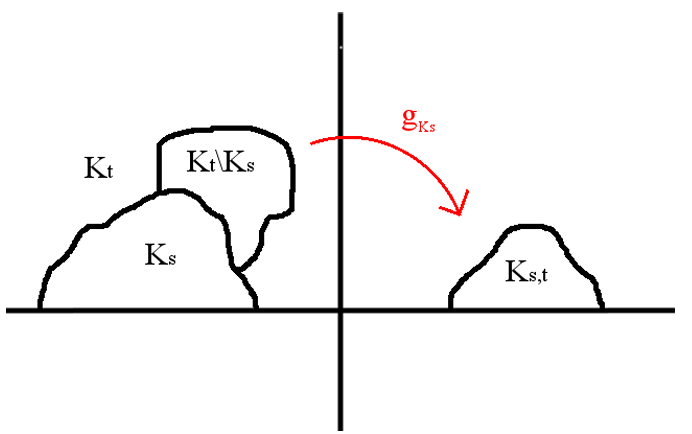
\includegraphics[width=0.5\linewidth]{Images/local SLE.png}
        \caption{A continuity Condition}
        \label{fig:enter-label}
    \end{figure}
    \item Parameterized by half plane capacity if $\hcap(A_t) = 2t$ for all $t\geq 0.$
        \end{enumerate}
        We denote $\cal A$ to be the families of $\bbH-$hulls which satisfy 1-3. 
\end{defn}

\begin{thm}
    Suppose that $(A_t)\in \cal A$ with $g_t = g_{A_t}.$ There exists some $U: [0, \infty) \to \bbR$ continuous such that 
    \[\partial_t g_t(z)= \frac{2}{g_t(z) - U_t}, \quad g_0(z) = z\] We call $U$ the Loewner driving function for $(A_t).$
\end{thm}
\begin{proof}
    Since $\cal A$ is locally growing, we know that $\cap_{s\geq t} \overline{g_t(A_s)}$ contains a single point (compact and decreasing). Calling the point $U_t.$ clearly $U_t$ is continuous in $t.$ We know by Proposition 20 that 
    \[g_A(z) = z + \frac{\hcap (A)}{z} + O\left(\frac{c\,\rad(A)\hcap (A) }{|z|^2}\right)\] Recall that $g_{A + x}(z)- x = g_{A}(z-x).$  Combining these two facts,
    \begin{align}
    g_A(z) = g_{A + x}(z + x) - x  = z + \frac{\hcap (A + x)}{z +x} + O\left(\frac{c\,\rad(A+x)\hcap (A+x) }{|z+x|^2} \right)    
    \end{align}
     Let $\epsilon>0.$ By the fact that $\cal A$ is parameterized by a half plane capacacity, we know that $g_t(A_{t + \epsilon \sm A_t}) = 2\epsilon.$ Let $0 \leq s \leq t,$ and call 
    $g_{s,t} := g_t \circ g_s^{-1}$ In the above, let $A = g_t(A_{t + \epsilon}\sm A_t)$ and $x = -U_t.$ Noting that  $\rad(A - U_t) = \rad(A) \leq \text{diam}(A)$, we apply the above equation to show that 
    \[g_{t, t + \epsilon}(z) = z + \frac{2\epsilon}{z - U_t} + 2\epsilon \,\text{diam}(g_t(A_{t  + \epsilon} \sm A_t))\,O(\frac{1}{|z - U_t|^2})\] Tautologically, 
    \begin{align*}
        \frac{1}{\epsilon}\left(g_{t+ \epsilon}(z)\right) - g_t(z) &= \frac{1}{\epsilon}\left((g_{t,t + \epsilon} - g_{t,t})\circ g_t(z)\right)\\
        &= \frac{2}{g_t(z) - U_t} + 2 \,\text{diam}(g_t(A_{t  + \epsilon} \sm A_t))\,O(\frac{1}{|g_t(z) - U_t|^2})\\
        &\xrightarrow[\epsilon \to 0]{} \frac{2}{g_t(z) - U_t}
    \end{align*}
    
\end{proof}

\subsection{The Schramm-Loewner Evolution}
\begin{defn}
    Suppose that $(A_t)$ is a random family in $\cal A$ encoded with the Loewner driving function $U.$ We say that $A_t$ satisfies the \textbf{conformal Markov property} if the following holds. For each $t \geq 0,$ define $\mathcal{F} = \sigma(U_s : s \leq t).$ Then 
    \begin{enumerate}
        \item Conditioning the left side on $\cal F_s,$ we have that 
        \[\{g_s(A_{s + t}) - U_t\}_{t \geq 0} =^d \{A_s\}_{s\geq 0}\]
        \item For each $r>0,$ $(rA_{t/r^2}) = ^d (A_t)$
    \end{enumerate}
\end{defn}

\begin{rem}
    With 1, we see that $(T_{t + s} - U_t)_{s \geq 0}$ has the same distribution as $U_s$ (given $\cal F_t$). Since $U$ has stationary independent increments and it is continuous, then there is some $\kappa \geq 0$ and $a \in \bbR$ such that $U_t = \sqrt{\kappa}B_t + at,$ where $B$ is a SBM. Hence, by two, 
    \[r U_{r\sm r^2} = \sqrt{\kappa}r B_{r/ r^2} + ra(t/ r^2) =\sqrt{\kappa}\tilde{B} + at/r =^d U_t,\] implying $a = 0.$
\end{rem}
\begin{thm}
    If $A_t$ satisfies the conformal Markov property, then there is some $\kappa\geq 0$ such that $U_t = \sqrt{\kappa}B_t$ where $B$ is a SBM.
\end{thm}

\begin{defn}
    We define $\SLE_\kappa$ to be the random family of hulls $A_t$ which are obtained by solving the Loewner equation with $U_t = \sqrt{\kappa B_t},$ where $B$ is a standard Brownian Motion. 
\end{defn}
\begin{exmp}
    If $\kappa = 0,$ then $U_t = 0,$ corresponding to the family $A_t = [0, 2\sqrt{ t}i],$ as we have seen. 
\end{exmp}

\begin{exmp}
    Solve the SDE:
    \[dX_t = -\frac{X_t}{1-t}dt + dB_t\].
    Consider a more general SDE 
    \[dX_t = f(t)X_tdt + g(t)dB_t.\] Define 
    \[\mu(t):= \exp\{-\int_0^s f(s)\,ds\}, \implies d\mu_t = -f(t)\mu_t \,dt\] Using Ito's product rule, 
    \begin{align*}
    d(\mu_t, X_t) &= d\mu_t \,X_t + \mu_t\,dX_t + d\langle \mu \rangle_t\,d\langle X\rangle_t\\
    &= -f(t)\mu_t\,dt \,X_t+ \mu_t(f(t)X_tdt + g(t)dB_t)\\
    &= \mu_t g(t)\,dB_t
    \end{align*}
    Integrating both sides yields
    \[\mu_t X_t  =\int_0^s \mu_s g(s) \,dB_s\]
    Implying that 
    \[X_t = \frac{1}{\mu_t}\int_0^s \mu_s g(s) \,dB_s\]
    Solving our specific example, 
    \[X_t = (1-t)\int_0^t \frac{1}{1-s}\,dB_s\]
\end{exmp}

\begin{exmp}
    Let $A_r$ be unit annulus with inner disk radius $e^{-r}.$ Let $\tau$ be the exit time from $A_r$ of a Brownian motion. What is 
    \[\bbP\{|B_\tau| = e^{-r}\}\]
$\Im$
    Consider $\varphi = \log z,$ which sends $A_r \mapsto V,$ the vertical strip with sides $0$ and $-r$ on the real axis. Consider the Dirichlet problem on $V.$ where, up to rescaling, we need 
    \[H: \begin{cases}
        \triangle H(u) = 0, \quad 0<|u|<r\\
        H(u) = 0, \qquad u = 0\\
        H(u) = 1, \qquad u = -r
    \end{cases}\]
    Thus, 
    \[H(u) = \frac{-u}{r}\]  Using the fact that harmonic measure and exit probabilities are the same, we realize that 
    \[f_V(w) = \frac{-\Re(w)}{r}\] is exit probability on the strip. Using the conformal invariance, and noting $A_r = \varphi^{-1}(V),$ we compute
    \[f_{A_r}(z) = f_V(\varphi(z)) |\varphi'(z)| = \frac{- \Re(\log(z))}{r}\frac{1}{z} = \frac{-\log |z|}{r}\frac{1}{z}\]
\end{exmp}

\begin{exmp}
    Show that 2-D Brownian motion is neighborhood recurrent.
    \begin{proof}
        Without loss of generality, we will show Brownian motion is neighborhood recurrent about zero and suppose $B_0 = z.$ Let $\epsilon>0$ and let $R>|z|>\epsilon>0.$ Let $r$ large such that $e^{-r} < \epsilon$ and define $A_r$ as before. We define $\tau_r$ to be the exit of the Brownian motion through the inner radius and $\tau_R$ to be the one through the outer. Still using $\varphi(z) = \log(z),$ we send $A_r\mapsto V,$ where $V = \{w: -r < \Re(w) < \log (R)\}.$ We need 
        \[H: \begin{cases}
        \triangle H(u) = 0, \quad r<|u|<R\\
        H(u) = 0, \qquad u = \log (R)\\
        H(u) = 1, \qquad u = -r
    \end{cases}\]
    Thus, 
    \[H(u) = \frac{-u + \log (R)}{-\log (r) + \log (R)}\] Thus, pulling back to $A_r,$ we see that 
    \[\bbP\{\tau_r < \tau_R\} = \frac{-\log |z| + \log(R)}{-\log (r) + \log (R)}\] Sending $R\to \infty$ and apply to the strong Markov property to conclude. 
    \end{proof}
\end{exmp}


\subsection{Stochastic Calculus}
\begin{thm}
Suppose $\varphi(t,x)$ is sufficiently smooth. Let $X_t$ be a Brownian motion. Then 
\[\partial \varphi(t,X_t) = \partial_t \varphi(t,X_t) dt + \partial_x \varphi(t,X_t)\,dX_t + \frac{1}{2}\partial_{xx}\varphi(t,X_t)d\langle X\rangle_t\]
\end{thm}



\begin{thm}
    (Levy's Characterization of Brownian Motion) Let $M_t$ be a continuous martingale with $M_0 = 0.$ Suppose $\langle M_t\rangle = t.$ Then $M_t$ is a Brownian motion.
\end{thm}


\begin{rem}
    Let $X = (B^1, \dots, B^d)$ be a $d-$dimensional Brownian motion, then define
    \[Z_t := \|X_t\|^2 = \sum_{i=1}^d (B_t^i)^2\] As an aside, let $\varphi(x)= x^2,$ then using Ito's formula,
    \[d(B_t^2) = 2B_t \,dB_t + dt  \iff B_t^2 = \int_0^t2B_s dB_s + dt\] Thus, 
    \[Z_t =Z_0 +  \sum_{i=1}^d \left(\int_0^t 2B^i_s\,dB_s^i\right) + dt\] We define 
    \[Y_t:= \sum \int_0^t \frac{1}{Z_s^\frac{1}{2}}B_s^i \,dB_s^i.\] We know that $Y_t$ is a continuous local martingale since it is an Ito integral. Moreover, 
    \begin{align*}
    \langle Y\rangle_t &= \left\langle \sum_{i=1}^d \int_0^t \frac{1}{Z_s^\frac{1}{2}}B_s^i \,dB_s^i\right\rangle_t    \\
    &= \sum_{i=1}^d\left\langle \int_0^t \frac{1}{Z_s^\frac{1}{2}}B_s^i \,dB_s^i\right\rangle_t\\
    &= \sum_{i=1}^d \int_0^t \frac{1}{Z_s}(B_s^i)^2 ds\\
    &= t
    \end{align*}
    Hence, by Levy's characterization, $Y_t$ is a Brownian motion.
    Thus, we expand
    \begin{align*}
        Z_0 + 2\int_0^t Z_s^\frac{1}{2} dY_s + dt &= Z_0 + 2\int_0^t Z_s^\frac{1}{2} \sum_{i=1}^d \frac{1}{Z_t^\frac{1}{2}}B_t^i \,dB_t^i + dt\\
        &= Z_t
    \end{align*}
    Equivalently, $dZ_t = 2Z_t^\frac{1}{2}dY_t + d\cdot dt,$ where we call $Z$ the \textbf{square Bessel process of dimension $d$} and write $Z_t \sim \text{BESQ}^d$.

    Letting $\phi(x) = x^\frac{1}{2},$ we apply Ito's formula to $Z_t$ and see that 
    \begin{align*}
    dZ_t^\frac{1}{2} &= \frac{1}{2}Z_t^\frac{-1}{2}dZ_t - \frac{1}{8}Z^\frac{-3}{2} \,d\langle Z\rangle_t\\
    &= \frac{1}{2}Z_t^\frac{-1}{2}(2Z_t^\frac{1}{2}dY_t + d\cdot dt) - \frac{1}{8}Z^\frac{-3}{2} (4Z_t \,dt)\\
    &= dY_t + \frac{d}{2}Z_t^\frac{-1}{2}\,dt-\frac{1}{2}Z_t^\frac{-1}{2}\,dt\\
    &= dY_t + (\frac{d-1}{2})Z_t^\frac{-1}{2}\,dt
    \end{align*}

Defining $U_t:= Z_t^\frac{1}{2},$ we see that 
\[dU_t = (\frac{d-1}{2})\frac{1}{U_t}\,dt + dY_t\] We call this the \textbf{Bessel SDE of dimension $d$} and write $U_t \sim \text{BES}^d$
\end{rem}
\begin{prop}
    Suppose $d\in \bbR$ and $U_t \sim \text{BES}^d.$
    \begin{itemize}
        \item If $d < 2,$ then $U_t$ hits $0$ a.s.
        \item If $d\geq 2,$ then $U_t$ does not hit $0$ a.s.
    \end{itemize}
    \end{prop}
\begin{proof}
    Consider $U_t^{2-d}.$ Using Ito's formula, 
    \begin{align*}
        dU_t^{2-d} &= (2-d)U_t^{1-d}\,dU_t + \frac{1}{2}(1-d)(2-d)U_t^{-d}d\langle U
\rangle_t\\
&= (2-d)U_t^{1-d}\left((\frac{d-1}{2})\frac{1}{U_t}\,dt + dY_t\right) + \frac{1}{2}(2-d)(1-d)U_t^{-d}\,dt\\
&= \frac{1}{2}(d-1)(d-2)U_t^{1-d}\frac{1}{U_t}\,dt + (2-d)U_t^{1-d}dY_t + \frac{1}{2}(1-d)(2-d)U_t^{-d}\,dt\\
&= (2-d)U_t^{1-d}dY_t
    \end{align*}
    Since this shows that $U_t$ is an Ito integral, then $U_t^{2-d}$ is a continuous martingale For any $a\in \bbR,$ we let $\tau_a = \inf\{t \geq 0 : U_t = a\}$ Thus, if $a\leq U_0 < b < \infty,$ then $U_{t\wedge \tau_a \wedge \tau_b}$ is a bounded continuous martingale, and so by the OST,
    \[U_0^{2-d} = \bbE[U_{\tau_a \wedge \tau_b}^{2-d}] = a^{2-d}\bbP\{\tau_a < \tau_b\} + b^{2-d}\bbP\{\tau_b < \tau_a\}\] Letting $a = 0$ for the $d< 2$ case, we have that as $b\to \infty,$ 
    \[\bbP\{\tau_b < \tau_0\} = \left(\frac{U_0}{b}\right)^{2-d} \to 0\] For $d>2,$ we write 
    \[\bbP\{\tau)a < \tau_b\} = \left(\frac{U_0}{b}\right)^{2-d} - \left(\frac{b}{a}\right)^{2-d} \bbP\{\tau_b < \tau_a\}\] Letting $a\to 0,$ the result becomes clear. For $d = 2,$ replace $U_t^{2-d}$ with $\log U_t$ and prove similar.  
\end{proof}
\begin{rem}
    Back to Loewner! Suppose $U_t = \sqrt{\kappa}B_t$ and $g_t$ solves
    \[\partial_t g_t(z) = \frac{2}{g_t(z) - U_t}.\] Letting $\gamma$ be the curve corresponded to the family of hulls encoded by $(g_t),$ for each 
     $x\in \bbR,$  define $V_t^x = g_t(x) - U_t.$ Letting $\tau_x = \inf\{t \geq 0 \mid V_t^x = 0\}$ be the first time a singularity in the curve is absorbed by the real axis, we see that by using Ito's formula,
     \[dV_t^x = \frac{2}{g_t(x) - U_t}\,dt - dU_t = \frac{2}{V_t^x}\,dt - \sqrt{\kappa}\,dB_t.\] Letting $Y_t = -B_t,$ we see that 
     \[d(V_t^x/\sqrt{k}) = \left(\frac{2}{\kappa}\right) \frac{\sqrt{\kappa}}{V_t}\,dt + dY_t.\] Thus, $V_t^x/\sqrt{\kappa} \sim \text{BES}^d,$ where 
     \[\frac{d-1}{2} = \frac{2}{\kappa} \implies d = 1 + \frac{4}{\kappa}\] Hence, 
     \[d \geq 2 \iff \kappa \leq 4\] and by Proposition 22, $\tau_x < \infty$ iff $\kappa >4.$
\end{rem}

\begin{prop}
    $\SLE_\kappa$ corresponds to a simple curve for $\kappa \leq 4,$ and it is self intersecting for $\kappa >4.$ 
\end{prop}
\begin{proof}
    We have seen in the previous remark that $\SLE_\kappa$  intersects $\partial \bbH$ iff $\kappa>4.$ Let $t>0$ be fixed. We claim that $\gamma'$ defined by $\gamma'(s):= g_t(\gamma(s + t)) - U_t$ is an $\SLE_\kappa$ curve. One can see this by the conformal Markov property. Thus, for $\kappa \leq 4,$ $\gamma'$ never intersects $\partial \bbH,$ and thus the curve $\gamma$ never intersects itself.
\end{proof}

Let $\kappa >4.$
\begin{rem}
    Let $0 < x < y,$ and define 
    \[g(x,y):= \bbP\{\tau_x = \tau_y\}\] be the probability both $x$ and $y$ are cut off from $\infty$ at the same time. Note that 
    \begin{itemize}
        \item $g(x,y) = g(1, \frac{y}{x})$ since $\SLE_\kappa$ is scale-invariant by assumption. Clearly, $\bbP\{\tau_1 < t\} \to 1$ as $t \to \infty. $ Also, $\bbP\{\tau_r < t\} \to 0$ as $r\to \infty.$ Hence, $g(1,r) \to 0$ as $r\to \infty$
    \end{itemize}
\end{rem}
\begin{defn}
    We say that two events are equivalent if they differ by an event of probability zero.
\end{defn}

\begin{lem}
    For fixed $r>1,$ the even $\{\tau_1 = \tau_r\}$ is equivalent to 
    \[E = \{\sup_{t< \tau_1} \frac{V_t^r - V_t^1}{V_t^1} < \infty\}\]
\end{lem}
\begin{proof}
    Suppose $E$ occurs. Then there is some $C>0$ such that 
    \[\frac{V_t^r- V_t^1}{V_t^1} \leq C \iff \frac{V_t^r}{V_t^1} \leq C + 1  \iff V_t^r \leq V_t^1 \cdot C'\] Taking $r\to \infty,$ we know that $V_t^1 \to 0$ as $t\uparrow \tau_1$ and hence $V_t^r \to 0$ as $t \uparrow \tau_1,$ and thus $\tau_r \leq \tau_1.$ Thus $r$ must be swallowed before $1.$ Hence, 
    \[E \subseteq \{\tau_1 \geq \tau_r\} = \{\tau_1 = \tau_r\}\cup \{\tau_1 > \tau _r\}\]

    For the other direction, let $M>0,$ then if we define 
    \[\sigma_M:= \inf\{t \geq 0 : \frac{V_t^r - V_t^1}{V_t^1} \geq M\},\] we have by definition that
    \[\bbP\{\tau_1 = \tau_r \mid \sup_{t <  \tau_1}\frac{V_t^r - V_t^1}{V_t^1}\geq M\}= \bbP\{\tau_1 = \tau_r \mid \sigma_M < \tau_1\}\] Consider the map $z \mapsto \frac{z}{V^1_{\sigma_M}}$. Clearly, $V_{\sigma_M}^1 \mapsto 1$ and since 
    \[\frac{V^r_{\sigma_M}}{V_{\sigma_M}^1} = M +1,\] then $V^1_{\sigma_r}\mapsto M+1.$ Hence, by the scale invariance, $g(1, r) = g(1, 1 + M).$ We start the new $\SLE_\kappa$ from $0$ at time $\sigma_M$ by the Strong Markov Property, we have that 
    \[\bbP\{\tau_1 = \tau_r \mid \sigma_M < \tau_1\} = g(1, 1 + M) \to 0 \qquad M \to \infty.\] Thus, 
    \[\bbP\{\tau_1 = \tau_r , E^c\} = 0\]
\end{proof}

\begin{lem}
Let $C\in (0,1). $We have that \[\bbP\{\sup_{t < \tau_1} \frac{V_t^r - V_t^1}{V_t^1} < \infty\} = \begin{cases}
        C, \qquad \kappa\in (4,8)\\
        0, \qquad \kappa  = 8
    \end{cases}\]
\end{lem}
\begin{proof}
    Let $Z_t = \log \left(\frac{V_t^r - V_t^1}{V_t^1}\right)$ Recall that $dV_t^x = \frac{2}{V_t^x}dt + \sqrt{\kappa}dB_t$
    
    Letting $d = 1 + \frac{4}{\kappa},$ then by Ito's formula, 
    \[dZ_t = \left((\frac{3}{2} -d) \frac{1}{(V_t^1)^2} + \left(\frac{d-1}{2}\right)\left(\frac{V_t^r - V_t^1}{(V_t^1)^2 V_t^r}\right)\right)\,dt - \frac{1}{V_t^1} \,dB_t\]

Thus, to turn the martingale part of $Z_t$ ($-\frac{1}{V_t}\,dB_t$) into a SBM, we perform a time change. Consider
\[\sigma(t) := \inf\{u \geq 0 : \int_0^u \frac{1}{(V_s^1)^2}\,ds = t\} \implies t = \int_0^{\sigma(t)}\frac{1}{(V_s^1)^2}\,ds  \implies dt = \frac{d\sigma(t)}{(V_{\sigma(t)}^1)^2}\]

Defining 
\[Y_t:= -\int_0^{\sigma(t)}\frac{1}{V_s^1}\,dB_s\] as a local continuous martingale, then 

\[\langle Y\rangle_t = \left\langle- \int_0^{\sigma(t)} \frac{1}{V_s^1}\,dB_s\right\rangle_t = \int_0^{\sigma(t)}\frac{1}{(V_s^1)^2}\,dt = t\] and by Levy's characterization of a Brownian motion is a SBM. 

Defining $\tilde{Z}_t$ such that $\tilde{Z}_t = Z_{\sigma(t)},$ we have that
\begin{align*}
    d\tilde{Z}_t &= dZ_{\sigma(t)}\\
    &= dZ_{\sigma(t)}\cdot d\sigma(t)\\
    &= \left((\frac{3}{2} -d) \frac{1}{(V_{\sigma(t)}^1)^2} + \left(\frac{d-1}{2}\right)\left(\frac{V_{\sigma(t)}^r - V_{\sigma(t)}^1}{(V_{\sigma(t)}^1)^2 V_{\sigma(t)}^r}\right)\right)\,d\sigma(t) - \frac{1}{V_{\sigma(t)}^1} \,dB_{\sigma(t)}\\
    &= \left((\frac{3}{2} -d) \frac{1}{(V_{\sigma(t)}^1)^2} + \left(\frac{d-1}{2}\right)\left(\frac{V_{\sigma(t)}^r - V_{\sigma(t)}^1}{(V_{\sigma(t)}^1)^2 V_{\sigma(t)}^r}\right)\right)(V_{\sigma(t)}^1)^2\,dt + dY_t\\
    &= \left((\frac{3}{2} -d) + \left(\frac{d-1}{2}\right)\left(\frac{V_{\sigma(t)}^r - V_{\sigma(t)}^1}{ V_{\sigma(t)}^r}\right)\right)\,dt + dY_t
\end{align*}

\end{proof}

    


\end{document}